\section{Discapacidad Auditiva}

La discapacidad auditiva es una condición que limita la capacidad de una persona para escuchar. Esta puede manifestarse en distintos niveles de intensidad, desde una pérdida leve de audición hasta la sordera total. Además, esta condición puede tener diversas causas, como factores genéticos o exposición prolongada a ruidos fuertes \cite{five}. Es importante destacar que, independientemente de su origen o grado, la discapacidad auditiva puede representar un desafío significativo en la vida diaria de quienes la experimentan, afectando su comunicación, educación e integración social \cite{six}. 


\subsection{Causas de la sordera}

La Federación Mundial de Sordos (WFD) reporta que en todo el mundo hay 70 millones de personas sordas, de las cuales 34 millones son niños. Además, se estima que alrededor de 3 de cada 1,000 bebés nacen con sordera \cite{six}. En este contexto, es importante destacar que la sordera en los niños puede manifestarse durante el período prenatal debido a diversos factores. Por ejemplo, hay mutaciones genéticas (hereditarias y no hereditarias) que pueden aumentar la probabilidad de sordera congénita. Asimismo, existen infecciones intrauterinas, como la rubéola o el herpes, que también pueden desencadenar la sordera en el feto. Otra causa común es la exposición a medicamentos por parte de la madre que pueden provocar diversas malformaciones \cite{seven}. 

La prematuridad de un bebé es también un factor que puede influir significativamente en el desarrollo de problemas auditivos. Concretamente, los bebés prematuros tienen un mayor riesgo de desarrollar sordera debido a la posibilidad de que sus oídos no hayan alcanzado su completo desarrollo al momento del nacimiento. Además, los bebés prematuros comúnmente experimentan enfermedades que aumentan la probabilidad de desarrollar sordera, como la hiperbilirrubinemia (ictericia grave). Por otro lado, durante el parto pueden surgir complicaciones que resultan en asfixia perinatal, evento que puede ocasionar daños al sistema auditivo y nervioso del recién nacido \cite{seven}.

Cabe destacar que la sordera no solo aparece durante el periodo prenatal o perinatal, sino que también puede manifestarse en cualquier etapa de la vida, incluyendo la infancia, la adolescencia y la edad adulta. En niños y jóvenes, infecciones recurrentes del oído (otitis media crónica) pueden provocar pérdida de audición si no se tratan adecuadamente. A su vez, la meningitis es una infección que también puede ocasionar daños en el nervio auditivo y, consecuentemente, resultar en pérdida auditiva. Finalmente, la exposición continua a ruidos fuertes puede dañar gradualmente la audición a lo largo del tiempo. Esto es especialmente relevante en los jóvenes y adultos que utilizan con más frecuencia audífonos a un volumen alto \cite{six}.


\subsection{Clasificación de la sordera}

Una persona sorda, según la Organización Mundial de la Salud (OMS), es aquella cuya capacidad auditiva no supera los 20 decibelios (dB) en ambas orejas \cite{six}. Sin embargo, es importante tener en cuenta que la sordera puede manifestarse en diferentes grados, los cuales dependen de la gravedad de la pérdida auditiva y de la ubicación específica del problema en el oído.

En términos de grado de pérdida auditiva, la sordera se puede clasificar en leve, moderada, grave y profunda. La pérdida auditiva leve se refiere a una persona que puede escuchar algunos sonidos relacionados con el habla, pero no puede escuchar susurros. A una persona con pérdida auditiva moderada le cuesta entender el habla a un volumen normal. Por otro lado, una persona con pérdida auditiva grave no escucha ningún sonido a volumen normal, solo puede oír sonidos fuertes. Por último, una persona con pérdida auditiva profunda (o con sordera total) no escucha nada, exceptuando algunos sonidos extremadamente fuertes \cite{eight}. 

Al considerar la ubicación de la pérdida auditiva, esta puede clasificarse en tres tipos principales: conductiva, neurosensorial o mixta. La pérdida auditiva conductiva ocurre cuando hay un bloqueo que impide el paso del sonido del oído externo al medio. En cambio, la pérdida auditiva neurosensorial ocurre cuando hay daño en el oído interno o en el nervio auditivo. Esto resulta en que los sonidos no puedan ser procesados y posteriormente transmitidos al cerebro de forma correcta. Finalmente, la pérdida auditiva mixta, como su nombre sugiere, involucra una combinación de factores tanto conductivos como neurosensoriales. Esto puede ser el resultado de múltiples condiciones que afectan tanto el oído externo como el interno \cite{eight}. 


\subsection{Impacto de la discapacidad auditiva en las personas}

Actualmente se reporta que el 80\% de personas sordas residen en países de bajos ingresos, como Guatemala. En estos países, las condiciones precarias dificultan el acceso a servicios de salud auditiva adecuados, así como a tecnologías de asistencia y educación especializada. Como resultado, es frecuente encontrar niños, jóvenes e incluso adultos con pérdida de audición no solo no tratada, sino también no diagnosticada \cite{six}.

La sordera no tratada, según Dave Cutten, puede obstaculizar el desarrollo lingüístico y comunicativo de los niños, lo que incluye impedimentos en el desarrollo del vocabulario y dificultades para comprender y utilizar el lenguaje de manera efectiva \cite{nine}. Es fundamental destacar que los niños con sordera identificada suelen aprender a comunicarse a través de la lengua de señas, lo que mitiga en gran medida estos problemas. Sin embargo, independientemente de si los niños con sordera aprenden lengua de señas o no, existe una brecha lingüística entre la comunidad sorda y la oyente que tiene implicaciones psicológicas significativas. Por ejemplo, las personas sordas tienden a sentirse excluidas, solas, frustradas, enojadas y avergonzadas debido a que no pueden socializar fácilmente con sus familiares, compañeros y miembros de sus comunidades. Además, esta situación puede afectar negativamente el bienestar emocional de las personas sordas, generando sentimientos de ansiedad, depresión y baja autoestima \cite{ten}.

En el caso de los adolescentes y adultos, la discapacidad auditiva puede provocar efectos psicológicos y emocionales similares a los descritos anteriormente. Además, esta condición puede influir negativamente en las oportunidades educativas y laborales de las personas, lo que a su vez puede conducir a una mayor exclusión y discriminación en la sociedad \cite{eleven}. Por ejemplo, en Guatemala, de las 10 escuelas para personas sordas, ninguna ofrece educación secundaria. Esto, a su vez, ocasiona una brecha educativa significativa para los adolescentes sordos, limitando así su futuro académico y profesional \cite{four}.


\subsection{Barreras y desafíos enfrentados por la comunidad sorda en Guatemala}

En 2007, Elizabeth Parks y Jason Parks realizaron un estudio con el objetivo de analizar la situación sociolingüística de la comunidad sorda en Guatemala. A través de entrevistas y encuestas, identificaron que menos del 50\% de los sordos guatemaltecos reciben educación especializada. Además, observaron un bajo nivel de alfabetización, así como un pobre dominio del español entre este grupo. Según los autores, esta situación se atribuye a la presencia limitada de solo diez escuelas para los veintidós departamentos del país. De estas diez, tres son instituciones privadas, lo que las vuelve inaccesibles para muchas familias debido a limitaciones monetarias \cite{four}. 

En cuanto a educación superior, según Edith Paz, únicamente dos universidades en Guatemala ofrecen servicios de intérpretes para estudiantes sordos, aunque estos servicios están limitados exclusivamente a los departamentos de computación. Es importante destacar que, si bien los estudiantes tienen la opción de contratar intérpretes privados, esta posibilidad está restringida a aquellos provenientes de familias de altos recursos. Debido a esto, muchas personas sordas encuentran dificultades para acceder a empleos con un salario digno. Por ejemplo, el salario promedio mensual para un guatemalteco es de Q2,000, sin embargo, las personas sordas suelen ganar –en promedio– menos de Q600 mensuales \cite{four}.



\section{Lengua de Señas}

La lengua de señas es un sistema de comunicación utilizado por personas sordas y con discapacidad auditiva. Este utiliza gestos, movimientos de las manos, expresiones faciales y posturas corporales para transmitir ideas y emociones \cite{twelve}. Es importante mencionar que, al igual que los idiomas hablados, las lenguas de señas varían considerablemente entre países, existiendo más de 300 variaciones en todo el mundo \cite{thirteen}.


\subsection{Historia de la lengua de señas}

La lengua de señas se desarrolló de manera independiente por la comunidad sorda para satisfacer sus necesidades comunicativas. Históricamente estigmatizada y mal entendida, era considerada un lenguaje de gestos simple hasta que investigaciones realizadas en 1960 por William Stokoe revelaron su capacidad para expresar ideas complejas y estructuradas \cite{RodriguezVelasquezSF}.

En el siglo XVIII, el Abad Charles-Michel de L’Epée fundó la primera escuela pública para sordos, marcando un cambio trascendental en la educación de esta comunidad, utilizando la lengua de señas como principal medio de enseñanza. Este avance no solo facilitó la comunicación y el aprendizaje, sino que también permitió que los sordos desempeñaran roles activos como educadores. La metodología de L’Epée se expandió internacionalmente, influyendo en la creación de escuelas y en el desarrollo de nuevas lenguas de señas \cite{RodriguezVelasquezSF}.

Durante los siglos XIX y XX, las lenguas de señas ganaron reconocimiento como sistemas lingüísticos completos y estructurados, capaces de expresar una gama completa de ideas y emociones. En el siglo XX, el reconocimiento de los derechos lingüísticos de las comunidades sordas se amplió significativamente, afirmando la importancia de las lenguas de señas como herramientas educativas y culturales esenciales \cite{RodriguezVelasquezSF}.

A raíz de la necesidad de comunicación en las comunidades sordas, cada país ha desarrollado su propia lengua de señas, integrando a menudo estructuras de lenguas de señas extranjeras, como el \textit{American Sign Language (ASL)}, así como señas locales únicas. Esto ha dado lugar a que cada país, e incluso regiones dentro de los mismos, tengan su propia lengua de señas con estructuras gramaticales y léxicos distintos \cite{RuizVilla2022}.

\subsection{Lengua de señas en la actualidad}

En la actualidad, la lengua de señas se está adaptando a un entorno globalizado y tecnológicamente avanzado, donde las necesidades comunicativas evolucionan constantemente. Estos cambios han impulsado la creación de legislaciones, políticas, formación de asociaciones y el desarrollo de nuevas tecnologías destinadas a minimizar las barreras comunicativas. Un ejemplo significativo es la iniciativa de las Naciones Unidas al proclamar el 23 de septiembre como Día Internacional de las Lenguas de Señas, enfatizando la importancia de estas lenguas \cite{Parada2022}.

Sin embargo, a pesar de estos avances, persisten desafíos significativos. La falta de estandarización de las lenguas de señas a nivel global requiere que las personas aprendan la lengua de señas específica de cada comunidad, lo cual impide la existencia de una forma de comunicación internacional uniforme \cite{RuizVilla2022}.

Además, la lengua de señas, a menudo catalogada como una lengua minoritaria, es aprendida solamente por una pequeña fracción de la población sin discapacidades auditivas. Esta limitada difusión crea una brecha de comunicación significativa, contribuyendo a la marginación de la comunidad sorda y limitando su participación plena en actividades sociales y económicas. Esto subraya la necesidad de una mayor educación y sensibilización sobre la lengua de señas para promover una verdadera inclusión \cite{MelendezLabrador2021}.

\section{Lengua de Señas de Guatemala (LENSEGUA)}

\subsection{Historia}

El primer registro de la utilización de la lengua de señas en Guatemala se remonta a la escuela Fray Pedro Ponce de León, establecida en la Ciudad de Guatemala en 1946 para la educación de niños y niñas sordas. Sin embargo, según Edith Paz, esta institución tenía una filosofía oralista que prohibía el uso de señas y gestos para la comunicación. A pesar de estas restricciones, los estudiantes desarrollaron, durante el transcurso de 20 años, un sistema de señas para comunicarse entre ellos tanto dentro de las aulas como en público. Esta lengua de señas (también conocida como GSM) fue evolucionando con el paso del tiempo, incorporando influencias de ``Señas Caseras''\footnote{Se conoce como ``Señas Caseras'' al sistema de comunicación que utilizan los niños sordos, que no han sido expuestos a la lengua de señas, con padres oyentes para poder comunicarse y desenvolverse en el ámbito familiar \cite{EnSenasCultura}.} provenientes de distintos departamentos del país y de sistemas similares utilizados en España, Cuba, Costa Rica, El Salvador y Estados Unidos \cite{four}\cite{Aroche2022} .

A finales del siglo XX, se inauguraron otras diez escuelas para los jóvenes con discapacidad auditiva. A diferencia de la Escuela Fray Pedro Ponce de León, todas estas fomentaban el uso de la lengua de señas. Entre ellas, dos enseñaban \textit{American Sign Language} (ASL), mientras que las otras una variación de la lengua de señas formalizada a finales de la década de los sesenta (GSM) \cite{four}. 

En el 2001, el Comité Pro Ciegos y Sordos de Guatemala, una institución privada no lucrativa pionera en la educación y rehabilitación de personas con discapacidad auditiva, en conjunto con otros colaboradores, publicó el primer manual oficial de la Lengua de Señas de Guatemala (LENSEGUA). Este manual representó un avance crucial en la estandarización y enseñanza de la lengua de señas, proporcionando un recurso esencial para los estudiantes, profesionales y la comunidad en general interesada en aprender este método de comunicación \cite{deLeon2021}. Sin embargo, cabe destacar que este manual no tomó relevancia hasta el 2021, cuando el Congreso de la República de Guatemala aprobó la ‘Ley que Reconoce y Aprueba la Lengua de Señas de Guatemala’ (Decreto Número 135-96). Esta ley, como indica su nombre, reconoce a LENSEGUA como un medio de comunicación compuesto por un conjunto de movimientos corporales y una gramática propia de las personas sordas. Asimismo, establece que el Ministerio de Educación debe promover la introducción de LENSEGUA al sistema educativo nacional \cite{two}.

El Decreto estableció que todas las instituciones públicas y privadas deben garantizar la inclusión de LENSEGUA como parte de su comunicación y servicios. Además, se promueve la educación bilingüe (español y LENSEGUA) en las escuelas que atienden a estudiantes sordos, asegurando así su derecho a una educación equitativa y accesible \cite{CongresoGuatemala2020}.

Este reconocimiento no solo valida a LENSEGUA como una lengua completa y estructurada, sino que también impulsa la creación de políticas y programas destinados a mejorar la accesibilidad en todos los aspectos de la vida pública para la comunidad sorda, desde la educación hasta el acceso a los servicios de salud y legales. El Decreto promueve la inclusión y asegura que las personas con discapacidad auditiva tengan acceso a la educación y la información en lengua de señas, libre de cualquier discriminación \cite{CongresoGuatemala2020}.


\subsection{Variaciones regionales}

Aunque LENSEGUA es reconocida como la forma predominante de comunicación para la comunidad sorda en Guatemala, existen variaciones regionales que reflejan la diversidad cultural y lingüística dentro del país. Estas diferencias incluyen, pero no se limitan a, cambios sutiles en el vocabulario y los gestos utilizados. Por ejemplo, según Edith Paz, mientras que la Ciudad de Guatemala, Cobán y Quetzaltenango muestran similitudes significativas, San Marcos presenta un sistema ligeramente diferente, el cual se inspira aún más en el ASL \cite{four}.


\subsection{Gramática y estructura}
La gramática y estructura de LENSEGUA reflejan una vasta complejidad lingüística que permite a los usuarios expresar una amplia gama de conceptos y emociones. Este sistema de comunicación es completo con su propia sintaxis, léxico y reglas gramaticales. Aquí se describen algunas de las características distintivas de LENSEGUA \cite{EnSenasCultura} \cite{EnSenasGramatica} \cite{EnSenasTecnicas}:

\begin{itemize}

    \item \textbf{Morfología}: La morfología en LENSEGUA utiliza modificadores manuales y no manuales para alterar el significado de los signos básicos, incluyendo modificaciones para indicar número, tiempo, aspecto, y otros atributos gramaticales.
    \begin{itemize}
        \item El signo para ``comer" podría modificarse para expresar ``comer mucho" mediante la repetición del signo o cambios en la expresión facial.
    \end{itemize}
    
    \item \textbf{Ausencia de género y artículos}: Como en muchas lenguas de señas, LENSEGUA no utiliza género gramatical ni artículos.
    \begin{itemize}
        \item Español: ``la casa'', ``el perro''.
        \item LENSEGUA signa ``casa'' y ``perro'' sin modificadores adicionales.
    \end{itemize}
    
    \item \textbf{No Uso de Preposiciones}: LENSEGUA omite preposiciones, que en español son cruciales para las relaciones espaciales o temporales. La relación se establece a través del contexto y la configuración de los signos.
    \begin{itemize}
        \item Español: ``en la casa''.
        \item LENSEGUA: se usa gesto para indicar la ubicación relativa y el signo de casa.
    \end{itemize}
    
    \item \textbf{Omisión de Signos de Puntuación y Mayúsculas}: LENSEGUA no utiliza signos de puntuación ni mayúsculas. La escritura refleja una secuencia continua de signos, que se diferencia notablemente de la estructura del español.
    \begin{itemize}
        \item LENSEGUA: ``Disculpar mi hija no llega colegio porque muy enferma tiene tos casa tomar medicinas''.
    \end{itemize}
    
    \item \textbf{Verbos No Conjugados}: En LENSEGUA, los verbos no se conjugan. El tiempo y el aspecto se indican con signos específicos al principio de la frase o a través de la expresión facial.
    \begin{itemize}
        \item Español: ``Yo estoy comiendo''.
        \item LENSEGUA: se signa ``yo comer''.
    \end{itemize}
    
    \item \textbf{Orden Gramatical}: El orden gramatical típico en LENSEGUA es Tiempo, Lugar, Sujeto, Objeto, Verbo (TLSOV), diferente al orden Sujeto, Verbo, Objeto (SVO) del español. Este orden facilita que el contexto temporal y espacial quede establecido claramente al inicio.
    \begin{itemize}
        \item Español: ``Yo ayer jugué futbol''.
        \item LENSEGUA: se signa ``ayer yo fútbol jugar''.
    \end{itemize}
\end{itemize}

\subsection{Aprendizaje y recursos}

LENSEGUA se puede aprender en varias instituciones y a través de recursos en línea que buscan facilitar el acceso y la difusión de esta lengua. Entre las principales entidades que ofrecen cursos y formación en LENSEGUA están \cite{LenseguaSF}:

\begin{itemize}
    \item ASEDES (Asociación Educativa para el Sordo)
    \item ASORGUA (Asociación de Sordos de Guatemala)
    \item Benemérito Comité Prociegos y Sordos de Guatemala
    \item En-Señas Guatemala
    \item CESGUA (Coordinación de Educación y Servicios en Guatemala)
    \item INTERGUA (Coordinación de intérpretes de lengua de señas de Guatemala)
    \item ANDYSISC (Servicios de interpretación profesional de Lengua de Señas)
    \item FUNDAL
    \item ONG Sordos Latinos Guatemala
\end{itemize}

Estas organizaciones no solo proporcionan educación en LENSEGUA, sino que facilitan una serie de conferencias y talleres impartidos por especialistas para personas con discapacidad auditiva \cite{LenseguaSF}.






% MODULO DE VISION POR COMPUTADORA ====



\section{Fundamentos de visión por computadora}

\subsection{Procesamiento de imágenes}
La visión por computadora es un campo de la inteligencia artificial que permite a las computadoras interpretar y comprender el contenido de las imágenes y videos.
Este campo se basa en la adquisición, procesamiento y análisis de imágenes digitales para extraer información significativa.
Los objetivos de la visión por computadora incluyen la automatización de tareas que requieren procesamiento visual, como el reconocimiento de objetos, la detección de patrones y el seguimiento de movimientos \cite{forsyth2012}.

\subsection{Técnicas básicas}
Los principios básicos de la visión por computadora incluyen técnicas de procesamiento de imágenes, como la mejora de imágenes, la segmentación de imágenes y la extracción de características.
La mejora de imágenes puede incluir el ajuste de contraste y eliminación de ruido.
La segmentación de imágenes se enfoca en la división de una imagen en partes significativas, con el objetivo de descartar información que no sea útil.
Por último, la extracción de características se enfoca en la identificación de elementos clave dentro de una imagen, como bordes o puntos de interés.
Estas técnicas son fundamentales para el desarrollo de aplicaciones que requieren una comprensión detallada de las imágenes \cite{aakanksha2020}.

\subsection{Herramientas}
En el ámbito de la visión por computadora, existen varias herramientas y bibliotecas de software que facilitan la implementación de técnicas de procesamiento de imágenes y análisis visual.
Entre las más utilizadas se encuentran OpenCV y MediaPipe.

Open Source Computer Vision Library (OpenCV) es una biblioteca de software libre de visión artificial y aprendizaje automático.
Esta proporciona más de 2500 algoritmos optimizados para realizar una amplia gama de tareas, como la detección y reconocimiento de rostros, la identificación de objetos, la clasificación de acciones en videos, el seguimiento de movimientos y la reconstrucción de estructuras 3D \cite{opencv2024}.

Desarrollado por Google, MediaPipe es un marco multiplataforma para la construcción de aplicaciones multimedia.
MediaPipe proporciona soluciones de vanguardia para la detección y seguimiento de manos, detección de rostros, entre otras.
Es particularmente útil para aplicaciones que requieren el seguimiento en tiempo real y la interacción basada en gestos \cite{google2024}.

Algo que estas dos herramientas tienen en común es el lenguaje de programación que se utiliza, ya que ambas son librerías de Python.
Python es un lenguaje de programación ampliamente utilizado en visión por computadora, especialmente cuando se combina con bibliotecas como OpenCV y MediaPipe.
Estas herramientas permiten a los desarrolladores implementar aplicaciones avanzadas de visión por computadora de manera eficiente y con buenos resultados.
La principal ventaja de utilizar estas librerías es que no se necesita entrenar los modelos de visión por computadora desde cero, ya que en muchos casos se puede utilizar uno de los modelos que forman parte de estas librerías \cite{altunay2019}.

\section{Aplicaciones de visión por computadora}

\subsection{Medicina}
La visión por computadora tiene una amplia gama de aplicaciones en diversos campos. 
En la medicina, se utiliza para el diagnóstico asistido por computadora, ayudando a los médicos a detectar enfermedades a partir de imágenes médicas como radiografías y resonancias magnéticas. 
Adicionalmente, puede ayudar a que los diagnósticos sean más certeros, ya que la tecnología puede servir como una segunda opinión del diagnóstico \cite{goldsmith2021}.

\subsection{Industria automotriz}
En el sector automotriz, la visión por computadora es fundamental para el desarrollo de vehículos autónomos y sistemas avanzados de asistencia al conductor. 
Estos sistemas dependen de la capacidad de los vehículos para identificar y responder a señales de tráfico, peatones y otros obstáculos en la carretera.

\subsection{Seguridad y vigilancia}
En el ámbito de la seguridad y vigilancia, la visión por computadora se utiliza para la detección de intrusos, el reconocimiento facial y la identificación de comportamientos sospechosos.
Estas tecnologías son fundamentales para la prevención de crímenes y la protección de la seguridad pública.

\subsection{Manufactura}
En el ámbito industrial, la visión por computadora se emplea para el control de calidad y la inspección automatizada de productos. 
Esto puede simplificar de manera drástica los procesos de manufactura, y reduce dramáticamente el tiempo requerido en procesos de control de calidad de los productos. 

\section{Redes neuronales}

\subsection{Fundamentos}
Las redes neuronales son un componente esencial de la inteligencia artificial.
El funcionamiento de estas se inspira en el funcionamiento del cerebro humano, con una gran cantidad de neuronas.
Estas redes están compuestas por capas de nodos, que son como neuronas artificiales, que procesan la información a través de conexiones ponderadas \cite{goodfellow2016}.

\subsection{Tipos de redes neuronales}
Existen varios tipos de redes neuronales, cada una adecuada para diferentes tareas.
Las redes neuronales feedforward (FNN) son las más simples, donde la información se propaga en una sola dirección, de la entrada a la salida.
Las redes neuronales convolucionales (CNN) son especialmente efectivas para el procesamiento de imágenes debido a su capacidad para reconocer patrones espaciales jerárquicos.
Por último, las redes neuronales recurrentes (RNN) son adecuadas para el procesamiento de datos secuenciales, como el reconocimiento de voz o la traducción automática \cite{ibm2024}.

\subsection{Aplicaciones en visión por computadora}
Las aplicaciones de redes neuronales en visión por computadora incluyen la clasificación de imágenes, donde las CNN pueden identificar y categorizar objetos dentro de una imagen, y la detección de objetos, donde se localizan y etiquetan múltiples objetos dentro de una escena.
Estas tecnologías son fundamentales para el desarrollo de sistemas avanzados de reconocimiento de señas, como el proyecto "Señas Chapinas: Traductor de LENSEGUA", que utiliza redes neuronales para interpretar el lenguaje de señas guatemalteco en tiempo real.

\section{Evaluación de modelos de visión por computadora}

\subsection{Matriz de confusión}
La matriz de confusión es una herramienta que permite visualizar el rendimiento de un modelo de clasificación. 
Se organiza en una tabla que muestra las predicciones del modelo en comparación con las verdaderas etiquetas de los datos. 
Esta matriz se compone de cuatro componentes principales:
\begin{itemize}
    \item Verdaderos Positivos (TP): Casos correctamente clasificados como positivos.
    \item Falsos Positivos (FP): Casos incorrectamente clasificados como positivos.
    \item Verdaderos Negativos (TN): Casos correctamente clasificados como negativos.
    \item Falsos Negativos (FN): Casos incorrectamente clasificados como negativos.
\end{itemize}

La matriz de confusión es una herramienta útil para evaluar el rendimiento de un modelo de clasificación, ya que proporciona información detallada sobre los errores del modelo \cite{ibm2024MC}.
Adicionalmente, la matriz de confusión se puede utilizar para calcular otras métricas de rendimiento del modelo, como la sensibilidad y la puntuación F1.

\subsection{Sensibilidad}
La sensibilidad, también conocida como \textit{recall}, es una métrica que mide la proporción de casos positivos que fueron correctamente identificados por el modelo.
Un alto valor de sensibilidad indica que el modelo tiene una buena capacidad para detectar la clase positiva, lo cual es especialmente importante en aplicaciones donde se desea minimizar los falsos negativos \cite{ML2024Recall}.
Se calcula utilizando la siguiente fórmula:

\begin{equation}
    \text{Sensibilidad} = \frac{TP}{TP + FN}
\end{equation}

Donde TP son los verdaderos positivos y FN son los falsos negativos.

\subsection{Puntuación F1}
La puntuación F1, más comúnmente conocida como F1-score, es una métrica que combina la precisión y la sensibilidad en un solo valor. 
Se utiliza para evaluar el equilibrio entre la capacidad del modelo para identificar casos positivos (sensibilidad) y la exactitud de esas identificaciones (precisión). 
Se calcula de la siguiente manera:

\begin{equation}
    \text{F1-score} = 2 \times \frac{\text{Precisión} \times \text{Sensibilidad}}{\text{Precisión} + \text{Sensibilidad}}
\end{equation}

Donde la precisión se calcula como:

\begin{equation}
    \text{Precisión} = \frac{TP}{TP + FP}
\end{equation}

Donde TP son los verdaderos positivos y FP son los falsos positivos.

La puntuación F1 es especialmente útil en situaciones donde hay un desbalance en las clases, ya que proporciona una medida más completa del rendimiento del modelo que la precisión o la sensibilidad por separado \cite{f1score}.
Esta métrica es ampliamente utilizada en la evaluación de modelos de clasificación.



% MODULO DE CHATPGPT y LAMDA ====

\section{Natural Language Processing (NLP)}

El \textit{natural language processing} (NLP), o procesamiento de lenguaje natural, es un campo de la inteligencia artificial que se enfoca en la comprensión y manipulación del lenguaje humano. Este campo no se limita a un solo modelo, sino que abarca una variedad de técnicas y algoritmos diseñados para interpretar y generar texto de manera efectiva \cite{fifteen}. Estos modelos se pueden utilizar en diversos contextos, desde análisis de sentimientos hasta traducciones automáticas, lo que demuestra su versatilidad y aplicación práctica en diferentes áreas de la tecnología y la comunicación \cite{sixteen}.


\subsection{Técnicas y fundamentos}

En NLP, el preprocesamiento del texto es una etapa en la cual se preparan y limpian los datos antes de aplicar técnicas de análisis más avanzadas. Este proceso incluye varias etapas, como la \textit{tokenización}. Esto consiste en dividir el texto en unidades más pequeñas, como palabras, con el fin de facilitar su posterior análisis. Además, el preprocesamiento también suele involucrar el \textit{stemming}, que consiste en reducir las palabras a su forma base o raíz. Esto ayuda a normalizar el texto y a eliminar las variaciones morfológicas. Por último, se suele llevar a cabo la eliminación de \textit{stopwords}, que son palabras comunes pero que no aportan un significado contextual importante al texto, como 'el', 'la', 'de' y 'en'. En algunos casos, cabe destacar que puede ser necesario realizar un preprocesamiento más exhaustivo. Por ejemplo, dependiendo de las necesidades, se puede considerar el manejo de sinónimos para reducir el vocabulario de un texto \cite{sixteen}.

Posterior al preprocesamiento, se puede aplicar \textit{text feature extraction}. Este término engloba diferentes métodos, como \textit{bag of words} y \textit{N-grams}. Sin embargo, todos tienen como objetivo crear estructuras de datos que permiten representar de manera adecuada la información contenida en el texto. Por ejemplo, \textit{bag of words} genera un listado de palabras que constituyen el vocabulario de un texto, acompañado de la frecuencia con la que cada palabra aparece. Esta información puede ser útil para identificar la importancia relativa de las palabras en un documento. \textit{N-grams}, por otro lado, es una técnica en la cual se generan secuencias de palabras de longitud N. Estas secuencias se pueden utilizar para identificar las relaciones y estructuras entre las palabras en un texto \cite{sixteen}.

Una vez realizado el preprocesamiento del texto y creado las estructuras de datos adecuadas, se puede introducir dicha información en un modelo (o arquitectura) para llevar a cabo una variedad de tareas. Estas pueden incluir el análisis de sentimientos y la generación de texto. El análisis de sentimientos busca comprender las emociones expresadas en el texto, determinando si son positivas, negativas o neutras. Por otro lado, la generación de texto implica crear contenido de manera automática, ya sea completando frases, resumiendo artículos o incluso generando respuestas a preguntas del usuario \cite{seventeen}.


\subsection{Modelos principales}

Existe una amplia variedad de modelos diseñados para llevar a cabo las tareas de procesamiento de lenguaje natural mencionadas anteriormente. La elección entre estos depende de varios factores, como la complejidad de la tarea, la disponibilidad y calidad de los datos, y los recursos computacionales disponibles. 

\subsubsection{Aprendizaje automático}

Entre uno de los modelos más simples está el clasificador \textit{Naïve Bayes}. Este es un modelo probabilístico que –como indica su nombre– emplea el teorema de Bayes. En otras palabras, funciona a través de determinar la probabilidad de que un cierto evento ocurra dado que otro evento ya ha ocurrido (asumiendo la independencia condicional). Para su funcionamiento correcto, este clasificador suele recibir el vocabulario y la frecuencia con la que aparecen las respectivas palabras. A partir de esta información, por ejemplo, se puede determinar la probabilidad de que un texto pertenezca a una clase específica, como 'positivo' o 'negativo', dadas las palabras que contiene. En la detección de spam, se puede calcular la probabilidad de que un correo electrónico sea spam o no, basándose en la frecuencia de ciertas palabras o características en el mensaje \cite{eighteen}.

La regresión logística, similarmente, es otro modelo utilizado en el aprendizaje automático para problemas de clasificación. A pesar de su nombre, la regresión logística se utiliza principalmente para problemas de clasificación binaria, donde el objetivo es predecir la pertenencia a una de dos categorías distintas. A diferencia del clasificador \textit{Naïve Bayes}, que se basa en la probabilidad condicional, la regresión logística utiliza una función logística para modelar la relación entre las variables de entrada y la probabilidad de pertenencia a una clase específica. Esto permite su aplicación en una variedad de tareas de NLP, donde se busca clasificar el texto en categorías específicas \cite{nineteen}.

\subsubsection{Aprendizaje profundo}

Por otro lado, los modelos de aprendizaje automático se caracterizan por la utilización de redes neuronales. Una red neuronal es un modelo, compuesto por nodos interconectados (o neuronas), capaz de aprender patrones complejos en datos. Estos modelos, debido a su arquitectura, son capaces de realizar una mayor cantidad de tareas relacionadas con NLP, como generación de texto, traducción automática, resumen de documentos, respuesta a preguntas, entre otras \cite{twenty}. 

Es importante destacar que para entrenar y utilizar eficazmente estos modelos es necesario realizar una etapa de transformación de los datos mediante el proceso de \textit{embedding}. El \textit{embedding} es un proceso que convierte palabras o frases en vectores numéricos, permitiendo a los modelos de aprendizaje automático comprender su significado y relación. Además, se utiliza el \textit{padding} para igualar la longitud de las secuencias de entrada, lo que facilita su procesamiento en los modelos \cite{twentyone}.

\begin{figure}[H]
  \centering
  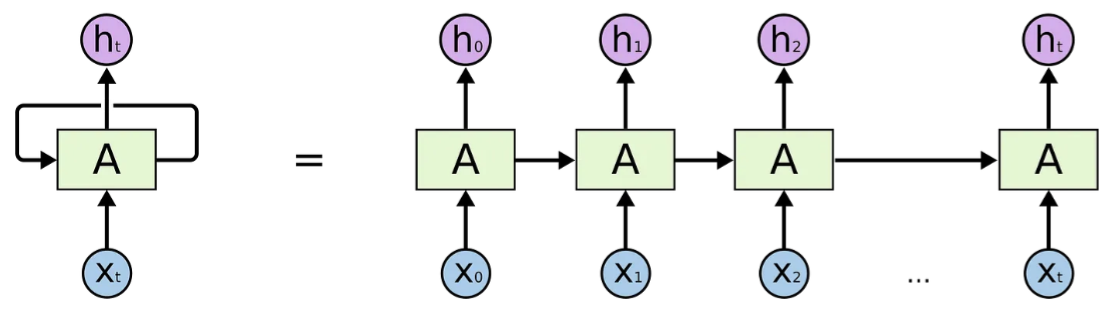
\includegraphics[width=0.5\linewidth]{figuras/RNN.png}
  \caption{Arquitectura de red neuronal recurrente.}
  \label{fig:RNN}
\end{figure}

Las \textit{recurrent neural networks} (RNN), o redes neuronales recurrentes, son comúnmente relacionadas con tareas de procesamiento de lenguaje natural. Estas redes trabajan con datos secuenciales, como series de tiempo o texto, debido a su capacidad para capturar dependencias entre los datos. Más específicamente, como se puede observar en la \ref{fig:RNN}, las capas de estas redes toman como entrada el dato actual a procesar así como la salida de la capa recurrente en el paso anterior. Esto les permite mantener un registro que se actualiza constantemente, y que –como resultado– les permite capturar información contextual a lo largo de una secuencia \cite{twentytwo}. Por tal motivo, estas redes neuronales pueden ser sumamente útiles para sistemas de autocompletado de texto, por ejemplo \cite{twentythree}. 

Una desventaja de los RNNs es que debido a su estructura recurrente pueden tener dificultades para capturar dependencias a largo plazo. Esto se debe a que la información se propaga a través de las diferentes capas, y en cada una se realizan transformaciones que pueden ocasionar que la información relevante se diluya o se pierda. Sin embargo, cabe destacar que existen arquitecturas RNN con ciertas modificaciones capaces de mitigar –hasta cierto punto– esta problemática, como las redes \textit{long-short term memory} (LSTM) \cite{twentythree}.

En general, las redes neuronales tradicionales tienen una limitación relacionada con la cantidad de información que pueden procesar y/o recordar. Sin embargo, existen otros tipos de modelos, como los los \textit{large language models} (LLMs), o modelos de lenguaje grande, que tienen la capacidad de superar estas limitaciones. Estos modelos específicos tienen la característica de poder ser entrenados con grandes cantidades de datos (millones). Esto, obviamente, les permite poder capturar patrones más complejos en el lenguaje, así como también generar texto con mayor coherencia \cite{twentyfour}.

\begin{figure}[H]
  \centering
  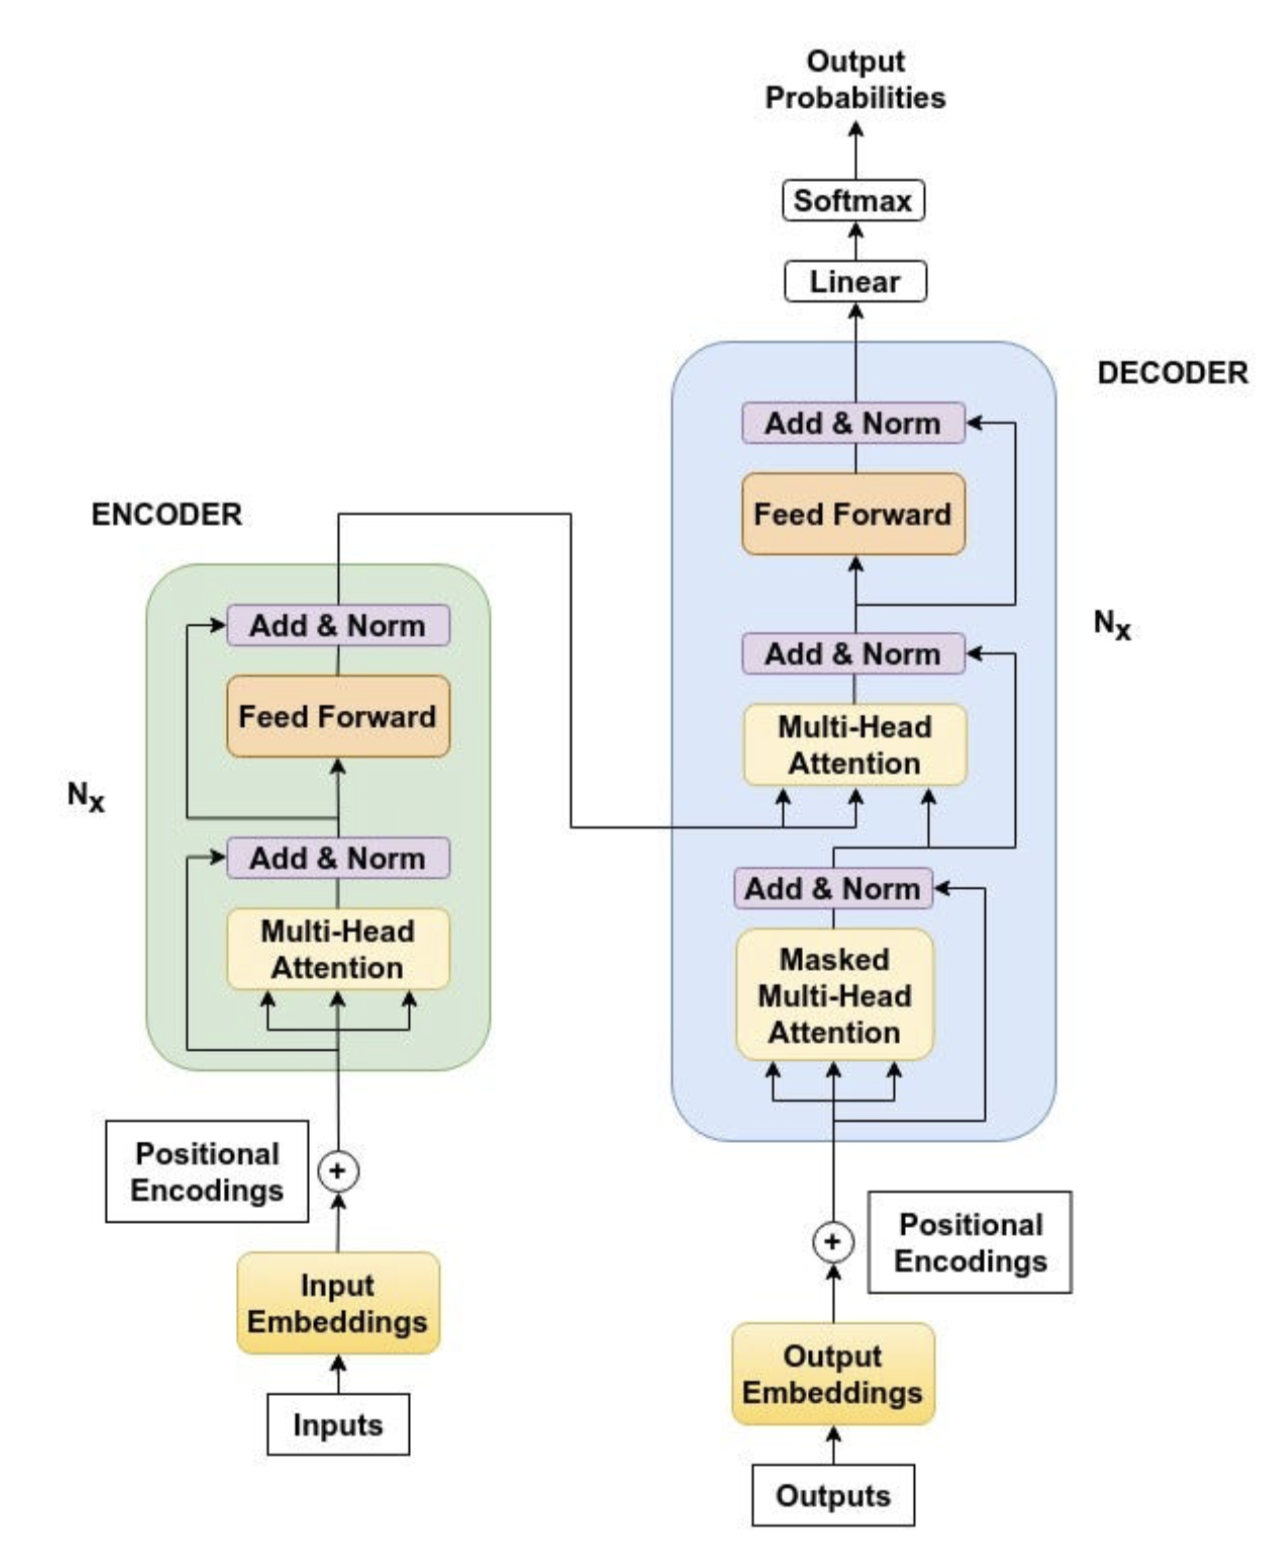
\includegraphics[width=0.5\linewidth]{figuras/TRANSFORMER.png}
  \caption{Arquitectura de transformer}
  \label{fig:TRANSFORMER}
\end{figure}

Una de las arquitecturas más utilizadas para los LLMs es la del transformador. Un transformador es una red neuronal compuesta, comúnmente, por un \textit{encoder} (codificador) y/o un \textit{decoder} (decodificador). El \textit{encoder} se encarga de procesar los \textit{tokens} de entrada, determinando cuál es la relevancia relativa de cada uno en su contexto. A través de esto, dicho componente es capaz de crear representaciones contextuales de cada \textit{token}. Por otro lado, el \textit{decoder} utiliza el resultado del \textit{encoder} para generar secuencias de salida. Sin embargo, en modelos que emplean únicamente \textit{decoders}, estos asumen la responsabilidad de procesar la entrada y generar la salida de forma simultánea \cite{twentyfive}.

Cabe destacar que el \textit{encoder} y \textit{decoder} están estructurados de una forma similar. Por ejemplo, como se puede observar en la \ref{fig:TRANSFORMER}, ambos tienen capas llamadas \textit{multi-head attention}, y \textit{feed forward}. Las capas de \textit{multi-head attention} le permiten al modelo poder enfocarse en diferentes partes de una secuencia simultáneamente, para así determinar cuál de todas es relevante. Por otro lado, las capas \textit{feedforward} representan capas ocultas que procesan los datos y permiten al modelo aprender patrones complejos en las secuencias de entrada \cite{twentysix}. 








\section{Arquitecturas basadas en transformadores}


\subsection{Generative Pre-trained Transformer (GPT)}

Existen diversos modelos que utilizan la arquitectura de transformadores. Sin embargo, uno de los más populares es el \textit{generative pretrained transformer} (GPT), o transformador generativo preentrenado. Este modelo fue presentado originalmente en el 2018 por OpenAI, en su artículo \textit{Improving Language Understanding by Generative Pre-Training}. En esta publicación, los autores describen detalladamente la arquitectura del GPT. Además, resaltan que al entrenar un modelo con extensas cantidades de texto, este adquiere conocimientos sobre el mundo real y desarrolla la capacidad de procesar dependencias a largo plazo. Esto resulta en que el GPT sea capaz de responder preguntas de cualquier índole, así como clasificar texto \cite{twentyseven}.

En la actualidad, este modelo se utiliza principalmente en un \textit{chatbot} desarrollado por OpenAI, conocido como ChatGPT. La versión gratuita de esta herramienta utiliza la tercera versión del modelo GPT para llevar a cabo interacciones conversacionales naturales con los usuarios. Este modelo fue preentrenado con más de 45 \textit{terabytes} (o 45,000 \textit{gigabytes}) de texto plano \cite{twentyeight}, en comparación con la versión piloto, que fue preentrenada únicamente con 40 \textit{gigabytes} \cite{twentynine}. 

\subsubsection{Arquitectura}

Un GPT, a diferencia de otros transformadores, se distingue por su uso exclusivo de decodificadores en su arquitectura. De hecho, emplea múltiples decodificadores apilados, los cuales dependen de la salida del decodificador anterior para generar texto coherente y relevante \cite{thirty}. Esta característica le permite al modelo capturar relaciones contextuales a diferentes niveles de abstracción, lo que, a su vez, le posibilita analizar y replicar el lenguaje natural \cite{thirtyone}.

\begin{figure}[H]
  \centering
  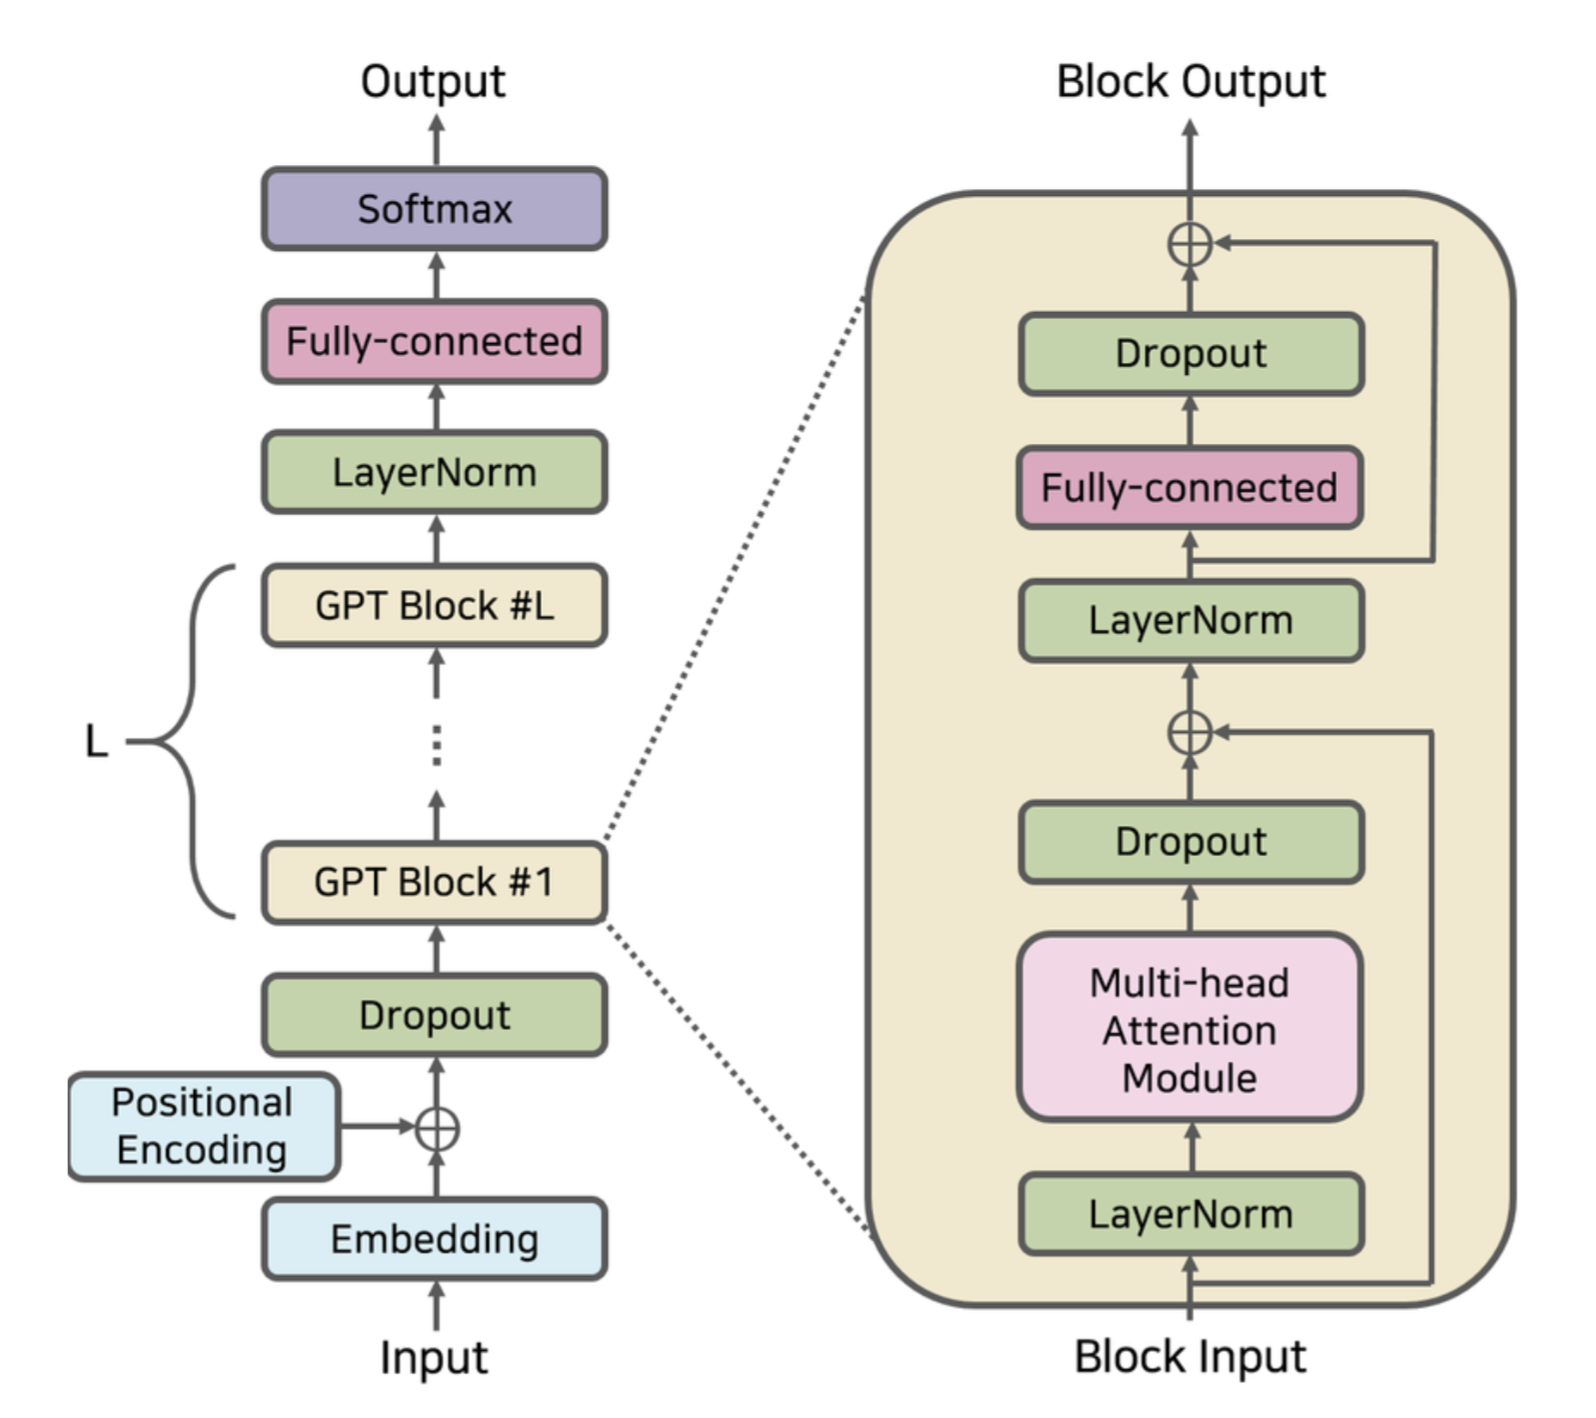
\includegraphics[width=0.5\linewidth]{figuras/GPT.png}
  \caption{Arquitectura de Generative Pre-trained Transformer (GPT).}
  \label{fig:GPT}
\end{figure}

Como se puede observar en la Figura \ref{fig:GPT}, la entrada de estos modelos primero pasa por una capa de \textit{embedding}. Como se mencionó en secciones anteriores, en este proceso se convierten las palabras o frases en vectores numéricos. Cabe destacar que la entrada está limitada a 2048 palabras, por lo cual también se utiliza \textit{padding} para ajustar las secuencias más cortas y asegurar una longitud uniforme antes de ingresarlas al modelo. Al concluir esa etapa, se continúa a la fase de \textit{positional encoding}, en la cual se asignan vectores de posición a cada vector numérico con el propósito de poder identificar su ubicación en la secuencia \cite{thirtytwo}.

Después de algunas capas variables, se procede a la utilización de los decodificadores apilados. Cabe destacar que todos están estructurados de una forma similar, conteniendo capas de normalización, \textit{dropout}, \textit{multi-head attention}, y \textit{fully connected} (o \textit{feed forward}). Posteriormente, el resultado del último \textit{decoder} se normaliza y se pasa a una capa oculta, seguido por una función \textit{softmax}. Esta última genera una distribución de probabilidad, la cual ayuda a identificar cuál es la próxima palabra más probable en la secuencia, según el contexto proporcionado por el modelo \cite{thirtytwo}.



\subsection{Large Language Model Meta AI (LLaMA)}

Otro modelo reconocido que se basa en la arquitectura de \textit{transformadores} es el \textit{Large Language Model Meta AI} (LLaMA), que fue desarrollado por Meta y lanzado a principios de 2023. Lo que diferencia a LLaMA de otros modelos es su diseño \textit{open source}, lo que permite que cualquier persona acceda a su código base y realice modificaciones o adaptaciones según sus necesidades. Además, LLaMA está optimizado para ser más eficiente en cuanto a recursos computacionales, lo que facilita su ejecución y entrenamiento en sistemas con menos capacidad. Esta eficiencia, combinada con su naturaleza de código abierto, lo convierte en una herramienta poderosa y accesible, especialmente para investigadores y desarrolladores con recursos limitados \cite{touvron2023llama}.

La versión más reciente de LLaMA, LLaMA 3.0, fue lanzada con significativas mejoras en su capacidad de procesamiento y versatilidad. Esta versión fue entrenada utilizando un total de 15 billones de \textit{tokens} de datos en múltiples idiomas, lo que le permite tener un rendimiento mejorado y adaptarse a un rango más amplio de tareas y contextos. Esta versión se ofrece en dos variantes principales: una versión con 8.000 millones de parámetros (8B) y otra más avanzada con 70.000 millones de parámetros (70B). Estas variantes permiten a los usuarios elegir el modelo que mejor se ajuste a sus necesidades, equilibrando precisión, rendimiento y eficiencia computacional \cite{touvron2023llama}.


\subsubsection{Arquitectura}

LLaMA, al igual que GPT, utiliza exclusivamente decodificadores en su arquitectura basada en transformadores. Su diseño incluye múltiples decodificadores apilados, los cuales trabajan en conjunto para procesar y generar texto coherente y contextual \cite{touvron2023llama}. Esta estructura modular le permite capturar relaciones complejas entre los \textit{tokens} en diferentes niveles de abstracción, lo que mejora su capacidad para analizar y replicar el lenguaje natural de manera eficiente.

Como se muestra en la Figura \ref{fig:LLaMA}, la entrada del modelo pasa inicialmente por una capa de \textit{embedding}, donde las palabras o frases se transforman en vectores numéricos para su procesamiento. Este paso incluye también la codificación posicional, la cual asigna vectores específicos que indican la ubicación de cada palabra en la secuencia, asegurando que el modelo pueda interpretar el orden y la estructura del texto \cite{touvron2023llama}.

Una vez que los vectores han sido generados y enriquecidos con la información posicional, estos se introducen en las capas de decodificadores apilados. Cada decodificador contiene submódulos como normalización (\textit{layer normalization}), \textit{dropout}, \textit{multi-head attention}, y redes \textit{feed-forward}. Este diseño permite al modelo refinar progresivamente la representación de los datos en cada capa, capturando patrones contextuales complejos \cite{touvron2023llama}.

Finalmente, el resultado de la última capa de decodificadores pasa por una capa oculta, seguida de una función \textit{softmax}, que genera una distribución de probabilidad para predecir la próxima palabra más probable en función del contexto \cite{touvron2023llama}.

\begin{figure}[H]
  \centering
  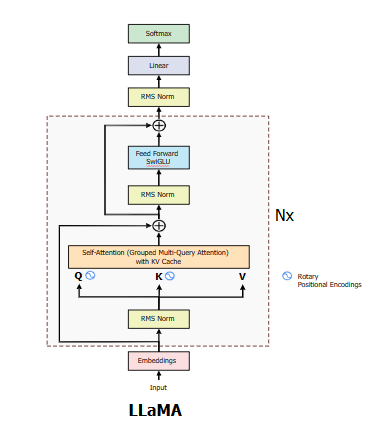
\includegraphics[width=0.65\linewidth]{figuras/LLAMA.png}
  \caption{Arquitectura de Large Language Model Meta AI (LLaMA).}
  \label{fig:LLaMA}
\end{figure}




\subsection{Métodos de entrenamiento y adaptación}  

\subsubsection{Pre-entrenamiento}  

Una vez definidas las arquitecturas de los modelos, es posible enseñarles a comprender, generar y procesar texto mediante técnicas avanzadas de aprendizaje. Este proceso inicia con el pre-entrenamiento, una etapa en la que los modelos aprenden patrones y estructuras del lenguaje sin enfocarse en una tarea específica. Para ello, se utilizan diversos datos, como artículos de prensa, libros, transcripciones de videos y audios \cite{twentynine}.

Durante el pre-entrenamiento, los modelos reciben frases incompletas como ejemplos y tienen la tarea de predecir la siguiente palabra o token en función del contexto. Si la predicción es incorrecta, el modelo ajusta internamente sus parámetros para priorizar las respuestas adecuadas en escenarios similares futuros. Al repetir este proceso de manera iterativa, ambos modelos adquieren la capacidad de generar texto coherente y relevante \cite{thirtytwo}.  

Es importante destacar que este tipo de modelos pueden ser posteriormente entrenados a través de \textit{fine-tuning} para adaptarse a tareas específicas, ampliando su utilidad y precisión en diferentes contextos.


\subsubsection{Fine-tuning}

\textit{Fine-tuning}, o ajuste fino, es un proceso a través del cual se adapta un modelo pre-entrenado para realizar una tarea nueva. Para esto, se le proporciona a un modelo ejemplos de entrada y salida relacionados a la tarea que se desea enseñar. Por ejemplo, para un traductor de idiomas, estas serían frases en el idioma de origen y la traducción correspondiente en el idioma destino. A partir de estos, el modelo ajusta los pesos de sus capas neuronales, los cuales son parámetros internos que determinan cómo se combinan las características de los datos de entrada para producir la salida. Este ajuste tiene como objetivo minimizar la diferencia entre las predicciones del modelo y los resultados reales, permitiendo que el modelo aprenda a resolver la nueva tarea de manera efectiva \cite{thirtythree}. 

Es importante mencionar que la cantidad de datos para el proceso de ajuste fino depende de la complejidad de la tarea. Para tareas simples puede ser suficiente decenas o cientos de ejemplos, mientras que para tareas más complejas se pueden necesitar miles o incluso millones de ejemplos para lograr un ajuste preciso del modelo. En otras palabras, a mayor complejidad usualmente se requiere una cantidad proporcionalmente mayor de datos \cite{thirtythree}.

\subsubsection{Prompt engineering}

En ciertos casos, los modelos pueden tener dificultades para aprender nuevas tareas a través del \textit{fine-tuning}, lo que puede resultar en respuestas incoherentes o inesperadas. Para abordar este tipo de problemas, se utiliza el \textit{prompt engineering}, una técnica que busca mejorar la formulación de las instrucciones dadas al modelo, de manera que interprete correctamente la tarea y genere respuestas más precisas. Más especificamente, esta técnica consiste en estructurar cuidadosamente las entradas, proporcionando ejemplos claros, instrucciones detalladas o indicaciones específicas sobre el formato y el contenido esperado. Esto permite guiar al modelo para que genere respuestas más consistentes y alineadas con los objetivos deseados \cite{thirtyfive}.

Una ventaja importante del \textit{prompt engineering} es que, en algunos casos, permite que el modelo realice nuevas tareas sin necesidad de un \textit{fine-tuning}. Sin embargo, para tareas más complejas, esta técnica por sí sola puede no ser suficiente. Por lo tanto, combinar \textit{prompt engineering} con \textit{fine-tuning} suele ser más efectivo. Mientras que el \textit{fine-tuning} adapta el modelo a tareas específicas, el \textit{prompt engineering} mejora la formulación de las instrucciones para optimizar el rendimiento. Utilizar ambas técnicas de manera complementaria maximiza las capacidades del modelo y mejora los resultados en tareas más desafiantes \cite{thirtyfive}.



\subsection{Métricas de rendimiento y evaluación}  

Para evaluar el rendimiento de un proceso de \textit{fine-tuning} o \textit{prompt engineering}, es fundamental utilizar métricas que permitan medir la similitud entre los resultados generados por un modelo y las respuestas esperadas. Estas métricas ayudan a identificar qué tan bien un modelo logra replicar o aproximarse al comportamiento deseado en tareas específicas. Algunas de las métricas más utilizadas son la distancia de Levenshtein y BLEU.

\subsubsection{Distancia de Levenshtein}

La distancia de Levenshtein mide el número mínimo de operaciones necesarias para transformar una cadena de texto en otra. Estas operaciones incluyen inserciones, eliminaciones y sustituciones de caracteres. Es una métrica útil para evaluar la similitud entre dos textos, ya que un menor valor indica una mayor cercanía entre ellos \cite{thirtynine}.


\subsubsection{Bilingual Evaluation Understudy (BLEU)}

La métrica BLEU (\textit{Bilingual Evaluation Understudy}) evalúa la calidad de un texto generado al compararlo con un texto de referencia, basándose en la coincidencia de \textit{n-gramas}. Estas coincidencias pueden ser unigramas, bigramas, trigramas, entre otros. BLEU también considera una penalización por brevedad, en caso de que los textos generados sean significativamente más cortos que el texto de referencia.

El valor de BLEU se expresa en una escala de 0 a 1, donde los valores más altos indican una mayor similitud entre el texto generado y el texto de referencia, reflejando una mejor calidad de generación \cite{bleu2001}.




\section{Explainable Artificial Intelligence (XAI)}

La Inteligencia Artificial Explicable (XAI), es un conjunto de técnicas que buscan hacer comprensibles las decisiones y predicciones de los modelos de inteligencia artificial. Esto resulta especialmente útil en modelos de \textit{deep learning} (como \textit{transformadores}) ya que estos sistemas, debido a su compleja arquitectura, funcionan como “cajas negras”. En otras palabras, el proceso mediante el cual se generan las predicciones no es fácilmente interpretable por los usuarios, lo que dificulta identificar cómo ciertas entradas llevan a un resultado específico \cite{doshi2017towards}.

Para abordar este desafío de interpretabilidad, las técnicas de XAI se han desarrollado siguiendo dos enfoques principales: intrínseco y \textit{post-hoc}. El enfoque intrínseco integra la explicabilidad en el diseño del modelo desde su creación, incorporando mecanismos de transparencia durante el proceso de desarrollo. Estos modelos se construyen con arquitecturas inherentemente interpretables, como árboles de decisión o reglas lógicas. Por otro lado, el enfoque \textit{post-hoc} ofrece interpretaciones tras el entrenamiento del modelo, sin alterar su estructura interna \cite{doshi2017towards}. Entre las herramientas \textit{post-hoc} más destacadas se encuentra LIME (\textit{Local Interpretable Model-agnostic Explanations}), que permite visualizar la contribución relativa de cada variable de entrada en las predicciones de un modelo, ayudando así a entender qué características tienen mayor influencia en los resultados generados \cite{dieber2020model}.


\subsection{Local Interpretable Model-agnostic Explanations (LIME)}

LIME es una técnica \textit{post-hoc} introducida por Ribeiro et al. en el 2016. Su principal característica es que puede aplicarse a cualquier tipo de modelo, lo que la hace \textit{model-agnostic}. Además, proporciona explicaciones locales, es decir, enfocadas en cada predicción individual \cite{ribeiro2016should}. 

Para generar estas explicaciones locales, LIME utiliza un proceso basado en la perturbación de los datos de entrada. La idea principal es crear múltiples versiones modificadas de los datos originales que se desean procesar para generar una predicción. Este proceso implica alterar sistemáticamente las características, ya sea variando valores numéricos o eliminando elementos. Por ejemplo, si se trabaja con características numéricas, las perturbaciones pueden consistir en variar los valores dentro de ciertos rangos o eliminarlos temporalmente. El objetivo es crear un conjunto de variaciones que permitan observar cómo el modelo responde a diferentes combinaciones de las características de entrada \cite{vu2019evaluating}.

Una vez generadas estas perturbaciones, cada entrada modificada se procesa a través del modelo original para obtener nuevas predicciones. Al comparar cómo cambia la salida del modelo para cada perturbación respecto a la predicción original, es posible determinar la importancia relativa de cada característica en la decisión final \cite{vu2019evaluating}. Este análisis permite identificar qué elementos de los datos de entrada tienen mayor influencia en las predicciones del modelo, revelando patrones y dependencias que no son evidentes a simple vista. Los resultados proporcionan una comprensión clara de cómo diferentes variables afectan el resultado final, lo que resulta fundamental para validar si el modelo está basando sus decisiones en características relevantes \cite{ribeiro2016should}. 










% MODULO DE ARQUITECTURA DE RED ==========

\section{Sistema Operativo: Linux Server}

\subsection{¿Qué es Linux?}
Linux es un sistema operativo de código abierto basado en Unix que se ha establecido como una opción poderosa y versátil para una variedad de plataformas, desde servidores y supercomputadoras hasta dispositivos móviles y electrodomésticos. Fue creado inicialmente por Linus Torvalds en 1991. El núcleo de Linux, conocido como el kernel, gestiona las interacciones del software con el hardware y es vital para la regulación de los recursos del sistema. A lo largo de los años, Linux ha ganado una popularidad masiva, en parte debido a su naturaleza de código abierto, que permite a los usuarios modificar y mejorar su software según necesiten. Además, su alta configurabilidad, estabilidad y robustez en seguridad lo hacen preferido en entornos empresariales y académicos. La comunidad de Linux es una de sus mayores fortalezas, contribuyendo constantemente con una amplia gama de distribuciones adaptadas a diferentes usos y preferencias \cite{Linux}.

\subsection{Historia de Linux}
Linux es un sistema operativo de código abierto creado en 1991 por Linus Torvalds, un estudiante de la Universidad de Helsinki. Inspirado en Unix, Torvalds deseaba ofrecer una alternativa gratuita y accesible, por lo que liberó Linux bajo la Licencia Pública General de GNU para permitir su uso, modificación y redistribución libre. Inicialmente adoptado por entusiastas tecnológicos y desarrolladores, Linux ha evolucionado hasta ser ampliamente utilizado en servidores, dispositivos móviles y supercomputadoras. Destacado por su estabilidad, seguridad y flexibilidad, es ahora uno de los sistemas operativos más predominantes a nivel mundial, con múltiples distribuciones como Ubuntu, Fedora y Arch que facilitan su uso en una gran variedad de entornos \cite{HistoriaLinux}.

\subsection{Linux Server}
Un servidor Linux se compone fundamentalmente de Linux, una familia de sistemas operativos de software libre y código abierto que se desarrollan alrededor del kernel de Linux. Originalmente creado como una versión alternativa y libre del sistema operativo MINIX, los servidores Linux se han popularizado gracias a su estabilidad, seguridad y flexibilidad. Estas características no solo los diferencian de sus contrapartes propietarias, sino que también mantienen bajos los costos de configuración y mantenimiento. Además, ofrecen una flexibilidad aumentada en la configuración, operación y mantenimiento de un servidor. Un sistema operativo de servidor Linux proporciona la interfaz central para la gestión de usuarios e implementa diversos servicios de seguridad y administración, todos cruciales para operar en una arquitectura cliente-servidor \cite{LinuxServer}.

\section{Virtualización}
La virtualización, en el contexto de la computación, implica la creación de versiones virtuales de recursos que originalmente eran físicos, como sistemas operativos y hardware de red. Este proceso permite a un solo servidor físico alojar múltiples máquinas virtuales (VMs), cada una con su propio sistema operativo y aplicaciones, operando de manera independiente pero compartiendo los recursos subyacentes del hardware físico \cite{Virtualizacion}.

El propósito principal de la virtualización fue maximizar la eficiencia del uso de recursos al permitir que múltiples sistemas operativos y aplicaciones se ejecutaran en un solo servidor físico. Esto no solo reduce los costos de hardware, sino que también aumenta la flexibilidad y la escalabilidad de los sistemas de TI. Las VMs pueden migrar entre servidores con mínimo tiempo de inactividad, lo que facilita el mantenimiento y la gestión del sistema \cite{Virtualizacion2}.

\section{Multipass}
Multipass es una herramienta ligera de virtualización diseñada para facilitar la creación y gestión de máquinas virtuales, enfocada especialmente en entornos de desarrollo y pruebas rápidas. Al integrarse de manera nativa con Ubuntu, Multipass permite desplegar y administrar múltiples instancias de Linux de manera eficiente, actuando como una mini-nube local en tu propio equipo. Multipass ha sido desarrollado con la simplicidad en mente, proporcionando una experiencia optimizada para usuarios que necesitan acceder rápidamente a entornos virtuales consistentes sin la complejidad de configuraciones avanzadas \cite{Multipass}.

\section{VPN}
\subsection{¿Qué es una VPN?}
Una VPN (red privada virtual) establece una conexión segura y privada entre dispositivos a través de Internet. Este tipo de red es fundamental para la transmisión de datos de manera segura y anónima a través de infraestructuras públicas. El proceso implica enmascarar las direcciones IP de los usuarios y cifrar la información transmitida, asegurando que solo las partes autorizadas puedan acceder y leer estos datos \cite{VPN}.

\subsection{¿Para qué sirven las VPNs?}
Las VPNs, o redes privadas virtuales, son esenciales para permitir conexiones remotas seguras a servidores y recursos de red. OpenVPN, un destacado software de VPN de código abierto, facilitó el establecimiento de redes locales virtuales entre computadoras dispersas geográficamente, permitiendo a los usuarios acceder y operar servidores y datos como si estuvieran físicamente presentes en la misma red local. Esto es crucial para empresas y organizaciones con equipos distribuidos, asegurando que la comunicación y el acceso a recursos críticos sean seguros y eficientes \cite{OpenVPN}.

\section{Arquitectura de base de datos}
\subsection{Bases de datos relacionales}
Una base de datos relacional es una estructura que organiza la información en filas y columnas dentro de tablas, facilitando el almacenamiento, la búsqueda y la gestión de datos de manera eficiente. Las tablas se enlazan entre sí mediante claves primarias y claves foráneas, creando relaciones que reflejan cómo se conectan los datos en diferentes tablas. Este sistema permite a los usuarios emplear consultas SQL para cruzar información de diversas tablas, proporcionando una herramienta poderosa para analizar y resumir el rendimiento empresarial \cite{Relacionales}.

\subsection{PostgreSQL}
PostgreSQL es una mejora del sistema de gestión Postgres, un prototipo avanzado de DBMS de próxima generación. Mientras conserva el modelo de datos potente y los tipos de datos ricos de Postgres, PostgreSQL ha reemplazado el lenguaje de consulta POSTQUEL por un subconjunto extendido de SQL, convirtiéndolo en una opción gratuita y de código abierto para el manejo de bases de datos. Desarrollado inicialmente en la Universidad de California en Berkeley, PostgreSQL ha evolucionado significativamente gracias a la contribución de un equipo de desarrolladores a nivel mundial \cite{Postgres}.

\subsection{Arquitectura de base de datos}
La arquitectura de datos se refiere al diseño estructural y a la metodología empleada para organizar y gestionar los recursos de datos en una organización o sistema. Este marco establece las políticas, normas y procedimientos para la recopilación, almacenamiento, manejo y uso de los datos con el fin de asegurar su accesibilidad, consistencia, integridad y seguridad. Una arquitectura de datos eficaz apoya la estrategia de información de una empresa, facilitando la integración y la operación de sistemas de TI, mejorando el soporte para las decisiones basadas en datos y optimizando el rendimiento de las aplicaciones \cite{ArquitecturaDatos}.

\section{APIs}
\subsection{¿Qué es una API?}
Una API (Interfaz de Programación de Aplicaciones) es un conjunto de reglas y especificaciones que las aplicaciones pueden seguir para comunicarse entre sí. Funciona como un puente que permite la interacción entre diferentes piezas de software de manera estandarizada. Por ejemplo, una aplicación de pronóstico del tiempo puede recibir datos de un servicio meteorológico utilizando una API para comunicarse con el sistema de dicho servicio \cite{API}.

\subsection{¿Cómo usar una API?}
Usar una API a nivel básico implica interactuar con un conjunto de definiciones y protocolos que permiten la comunicación entre diferentes componentes de software. Primero, es esencial entender los métodos estándar que la API ofrece, como obtener, crear, actualizar o eliminar recursos. Cada interacción sigue un patrón predefinido, facilitando así la integración y uso de la API en proyectos \cite{UsoAPI}.

\subsection{Implementar APIs a bases de datos}
Al desarrollar una aplicación que necesite interactuar con una base de datos mediante una API, puedes realizar operaciones como crear, recuperar, actualizar o eliminar registros. Estas operaciones se definen claramente con ciertos parámetros de entrada esperados y formatos de respuesta, lo que facilita la integración de sistemas complejos \cite{ImplementarAPI}.

\subsection{Implementar APIs para recepción y devolución de datos}
El uso de una API para enviar y recibir información implica interacciones estructuradas mediante solicitudes y respuestas definidas. Un ejemplo común es usar un método HTTP POST para enviar datos a la API, que luego devuelve una respuesta indicando éxito o fallo \cite{ImplementarAPIDatos}.

\subsection{¿Qué es Crontab?}
`Crontab` es una herramienta en sistemas Unix/Linux que permite la programación de tareas automatizadas que se ejecutan a intervalos específicos. Estas tareas, conocidas como cron jobs, son útiles para ejecutar scripts y comandos de forma recurrente sin intervención manual, lo cual es ideal para tareas de mantenimiento o procesamiento automatizado, como el reinicio de rachas en nuestra aplicación \cite{HostingerCrontabTutorial}.

\section{Bases de diseño y filosofía de DARPA}
Entre los conceptos fundamentales aplicados en el diseño de la arquitectura del sistema, se adoptaron varios principios expuestos en el documento "The Design Philosophy of the DARPA Internet Protocols" \cite{DARPA}. A continuación, se destacan los siguientes conceptos clave:

\subsection{Costo-efectividad y control}
La arquitectura de Internet, según lo planteado por DARPA, enfatiza la necesidad de manejar los recursos de manera eficaz bajo control administrativo distribuido. Esto justifica la decisión de utilizar servidores propios en lugar de servicios en la nube para este proyecto, reduciendo dependencias externas y costos operativos. Al mantener un control directo sobre la infraestructura, se puede gestionar de manera más eficiente el uso de los recursos, optimizando la relación costo-beneficio sin sacrificar el rendimiento.

\subsection{Flexibilidad y adaptabilidad}
La filosofía de diseño también subraya la importancia de adaptarse a diferentes entornos y requisitos técnicos. En este proyecto, la elección de Ubuntu como sistema operativo refleja un compromiso con un sistema flexible y robusto, ya que permite una personalización extensa. Aunque inicialmente se consideró el uso de RAID para la gestión del almacenamiento, se decidió desinstalarlo y desconfigurarlo debido a las limitaciones específicas del entorno de este proyecto. Esto asegura que la infraestructura sea adaptable a las necesidades actuales, manteniendo un enfoque simplificado en la gestión de recursos.

\subsection{Seguridad y privacidad}
Siguiendo los principios de diseño de DARPA, la seguridad es una prioridad fundamental. La integridad y seguridad de la comunicación entre los sistemas es vital para el éxito del proyecto. En este sentido, la implementación de una VPN segura mediante OpenVPN garantiza la protección de los datos transmitidos, asegurando que el acceso remoto y la transferencia de información se realicen de manera segura y confiable, reduciendo el riesgo de vulnerabilidades y ataques.

\section{Pruebas de eficiencia y de extremo a extremo en el servidor mediante APIs}

\subsection{¿Qué es una prueba de eficiencia?}
Las pruebas de eficiencia miden cómo el servidor responde bajo condiciones de carga habitual, evaluando aspectos como el tiempo de respuesta, la utilización de recursos (CPU, memoria y disco), y la capacidad del sistema para gestionar solicitudes simultáneas sin afectar negativamente el rendimiento. Estas pruebas permiten identificar oportunidades de optimización y ajustar la infraestructura para garantizar un rendimiento óptimo en condiciones normales de operación \cite{E2ETestingOverview}.

\subsection{¿Qué es una prueba de extremo a extremo (E2E)?}
Las pruebas de extremo a extremo (E2E) verifican el funcionamiento integral de la aplicación, evaluando cómo interactúan todos sus componentes en un flujo completo desde el punto de vista del usuario. Estas pruebas son esenciales para asegurarse de que cada parte de la aplicación, incluidas las APIs, funcione como se espera y que todos los puntos de interacción respondan adecuadamente dentro del sistema.

\begin{itemize}
    \item \textbf{Objetivo:} Confirmar que todas las partes de la aplicación operan de manera integrada, verificando que los flujos de trabajo completos (como registro, autenticación, envío de datos y consulta de información) se ejecuten sin errores.
    \item \textbf{Resultado esperado:} Que la aplicación realice todas las operaciones y flujos clave sin problemas, asegurando que cada funcionalidad principal esté correctamente integrada y funcione en conjunto.
\end{itemize}

\subsection{Impacto de la eficiencia y de las pruebas de extremo a extremo en el servidor}

\begin{itemize}
    \item \textbf{Eficiencia:} Un servidor eficiente maximiza el uso de los recursos disponibles, lo que permite reducir los costos operativos y mantener un rendimiento constante. Esto es esencial para asegurar tiempos de respuesta rápidos y garantizar que el sistema pueda manejar múltiples solicitudes concurrentes sin una degradación del servicio.

    \item \textbf{Pruebas E2E:} Las pruebas de extremo a extremo permiten validar el flujo completo de operaciones, asegurando que cada componente del sistema funcione correctamente y en sincronía. Estas pruebas ayudan a identificar cualquier posible problema de integración entre APIs y otros módulos de la aplicación, lo que es esencial para una experiencia de usuario fluida y un sistema robusto.
\end{itemize}

\section{Herramientas para pruebas de eficiencia y de extremo a extremo}

Para realizar las pruebas de eficiencia y extremo a extremo, se emplearon las siguientes herramientas:

\begin{itemize}
    \item \textbf{Python:} Se utilizó para desarrollar scripts personalizados que permiten simular múltiples usuarios y escenarios de carga en la aplicación, evaluando el tiempo de respuesta, el rendimiento y el uso de recursos en situaciones de carga típica y bajo prueba de integración completa \cite{PythonTesting}.
    \item \textbf{NGINX Amplify:} Herramienta de monitoreo utilizada para supervisar el uso de recursos en tiempo real, como CPU, memoria y tráfico de red. NGINX Amplify proporciona métricas detalladas y facilita el análisis de rendimiento durante las pruebas, identificando posibles áreas de optimización y problemas de integración \cite{NGINXAmplifyMonitoring}.
\end{itemize}

\subsection{Monitoreo del sistema}
\begin{itemize}
    \item \textbf{htop}: Proporciona una vista en tiempo real del uso de CPU, memoria y procesos en ejecución.
    \item \textbf{dstat}: Genera estadísticas combinadas de CPU, disco, memoria y red.
    \item \textbf{iotop}: Muestra el uso de disco por cada proceso, facilitando la identificación de procesos que consumen muchos recursos.
    \item \textbf{Prometheus}: Sistema de monitorización para métricas a gran escala.
    \item \textbf{Prometheus-Exporter}: Herramienta para monitorear las solicitudes entrantes al servidor.
    \item \textbf{Grafana}: Plataforma de visualización de métricas, utilizada para analizar los resultados de Prometheus \cite{MonitoringTools}.
\end{itemize}

\subsection{Pruebas de carga y end to end}

Las pruebas de carga se centran en medir la respuesta del sistema bajo condiciones de uso previstas, simulando múltiples usuarios y solicitudes simultáneas. Estas pruebas permiten evaluar el rendimiento, tiempos de respuesta y estabilidad del sistema cuando procesa diversas acciones en paralelo \cite{LoadViewLoadTesting}.

\begin{itemize} 
\item \textbf{Objetivo:} Evaluar cómo responde el sistema bajo una carga esperada de usuarios o solicitudes simultáneas, enfocándose en el rendimiento y la estabilidad mientras se procesan múltiples acciones. \item \textbf{Resultado esperado:} Que el sistema mantenga tiempos de respuesta y niveles de rendimiento aceptables bajo condiciones de uso normales (es decir, el número máximo de usuarios esperados en condiciones típicas). 
\item \textbf{Prueba:} La prueba de carga implementada simula a varios usuarios ejecutando operaciones simultáneas, como autenticación, envío de videos y marcación de favoritos. Se registra el tiempo de respuesta y el estado de cada acción, evaluando así la capacidad de la aplicación para manejar un volumen esperado de usuarios sin degradar su rendimiento. 
\end{itemize}

Las pruebas de Extremo a Extremo (E2E) se orientan a evaluar el flujo completo de la aplicación desde la perspectiva del usuario. A diferencia de las pruebas de carga, estas pruebas verifican que todos los componentes del sistema funcionen conjuntamente como se espera en un caso de uso completo.

\begin{itemize} 
\item \textbf{Objetivo:} Confirmar que todas las partes de la aplicación funcionan de manera integrada y que los componentes interactúan correctamente en un flujo de uso completo. \item \textbf{Resultado esperado:} Que la aplicación ejecute todas las operaciones y flujos clave sin errores (por ejemplo, registro, autenticación, envío y consulta de datos), asegurando que las funcionalidades principales se integren de manera adecuada. 
\item \textbf{Prueba:} La prueba E2E implementada cubre un caso de uso completo, desde la creación de un usuario hasta la interacción con las principales funciones de la aplicación, como autenticación, carga de videos, traducción y manipulación de favoritos. Esta prueba garantiza que cada parte del sistema funcione en conjunto en el flujo real de un usuario. 
\end{itemize}












% MODULO DE DISEÑO ==========
\section{Diseño de Interfaz de Usuario (UI)}
\subsection{Definición de UI (Interfaz de Usuario)}
El diseño de la interfaz de usuario (UI por sus siglas en ingles, \textit{User Interface}) se dedica a la creación de los elementos visuales e interactivos de un producto digital. En esencia, se trata de diseñar lo que los usuarios ven en sus pantallas \cite{OrtegaSF}.

La interfaz de usuario determina en gran medida las primeras impresiones que tienen estos acerca de un negocio o producto. Cuando los usuarios pueden navegar fácilmente por una interfaz y completar las tareas deseadas, no solo mejora su experiencia, sino que también beneficia al negocio en general. Cuanto más visualmente atractiva y acogedora sea una interfaz, más probable es que atraiga a los usuarios y los motive a explorar más \cite{OrtegaSF}.

\subsection{Elementos de la Interfaz de Usuario}
Los elementos de la UI son los componentes básicos de las aplicaciones y sitios web con los que los usuarios interactúan. Estos elementos son esenciales para el desarrollo de funcionalidades óptimas y una experiencia de navegación agradable. Los elementos UI se agrupan en tres categorías principales \cite{OrtegaSF}:

\begin{itemize}
    \item \textbf{Elementos de entrada}: Permiten a los usuarios ingresar información en el sistema y, en ocasiones, son parte del proceso de validación de entrada. Los elementos de entrada más comunes incluyen \cite{OrtegaSF}:
    \begin{itemize}
        \item Listas desplegables
        \item Campos de texto o contraseña
        \item Selectores de fecha
        \item Casillas de verificación
        \item Diálogos de confirmación
    \end{itemize}
    \item \textbf{Elementos de salida}: Muestran los resultados basados en las entradas del usuario y las operaciones previas. Ejemplos de elementos de salida son \cite{OrtegaSF}:
    \begin{itemize}
        \item Alertas
        \item Mensajes de éxito
        \item Mensajes de error
    \end{itemize}
    \item \textbf{Elementos auxiliares}: Proporcionan información adicional al usuario y mejoran la navegación. Estos elementos se dividen en tres subcategorías \cite{OrtegaSF}:
    \begin{itemize}
        \item \textbf{Elementos de navegación}: Facilitan el desplazamiento a través del producto digital \cite{OrtegaSF}. Algunos ejemplos son:
        \begin{itemize}
            \item Menús de navegación
            \item Listas de enlaces
        \end{itemize}
        \item \textbf{Elementos informativos}: Incluyen referencias que ayudan a utilizar o comprender el producto digital \cite{OrtegaSF}. Ejemplos son:
        \begin{itemize}
            \item Iconos
            \item Notificaciones
        \end{itemize}
        \item \textbf{Elementos de grupos o contenedores}: Ayudan a organizar y mantener los componentes del producto juntos \cite{OrtegaSF}. Ejemplos incluyen:
        \begin{itemize}
            \item Barras laterales
            \item Contenedores de contenido
        \end{itemize}
    \end{itemize}
\end{itemize}

\subsection{Estándares de Diseño}
\subsubsection{Tamaño y Posición de Botones}
El tamaño de los objetos táctiles en una aplicación móvil es crucial, ya que afecta directamente la facilidad con la que los usuarios pueden interactuar con la interfaz. Si los botones no tienen un tamaño y espacio óptimos, los usuarios podrían no alcanzar su objetivo o presionar el botón equivocado \cite{Bustos2022}.

Investigaciones sobre el tamaño y el espaciado de los botones han establecido estándares que funcionan para la mayoría de los usuarios. Los estudios encontraron que los usuarios tienen la menor precisión táctil en botones de menos de 42 píxeles, los cuales se usan generalmente para funciones de baja prioridad. La mayor precisión se encontró en botones de entre 42 y 72 píxeles. Por ello, se utilizan botones de aproximadamente 60 píxeles para funciones de prioridad media, mientras que los de más de 72 píxeles se reservan para funciones de alta prioridad, asegurando así la accesibilidad para todos los usuarios \cite{Anthony2019}.

\begin{figure}[H]
    \centering
    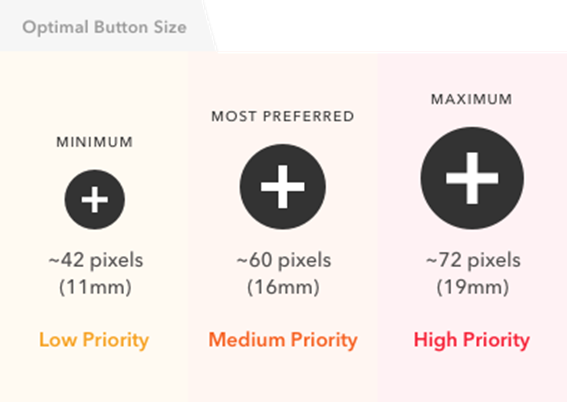
\includegraphics[width=0.6\linewidth]{figuras/optimal_button_size.png}
    \caption{Tamaño óptimo de botones según su prioridad}
    \label{fig:botones_optimos}
\end{figure}

Además del tamaño, existen ciertos márgenes y áreas táctiles recomendadas alrededor de los botones para garantizar que sean fácilmente accesibles y utilizables. Estos márgenes aseguran que haya suficiente espacio alrededor de los botones para evitar errores de pulsación. Dependiendo del tamaño del botón, se recomienda un margen de 12 a 24 píxeles para botones grandes, de 24 a 36 píxeles para botones medianos y de 36 a 48 píxeles para botones pequeños \cite{Anthony2019}. 

\begin{figure} [H]
    \centering
    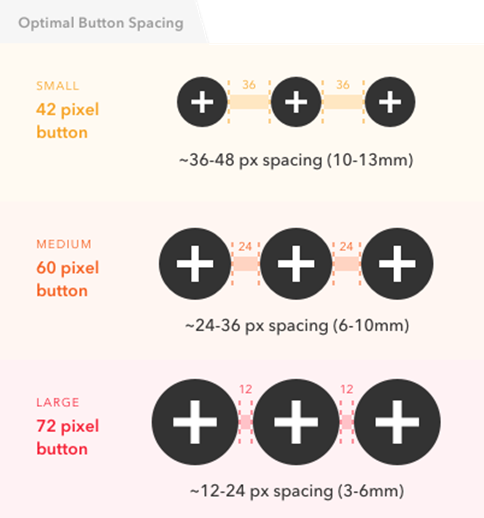
\includegraphics[width=0.5\linewidth]{figuras/optimal_space_buttons.png}
    \caption{Espaciado óptimo de botones según su tamaño}
    \label{fig:esapcio_optimo}
\end{figure}

Asimismo, la ubicación de los botones es fundamental para la usabilidad. Los usuarios están acostumbrados a interactuar con dispositivos digitales a lo largo del día y tienden a buscar ciertos elementos en ubicaciones predecibles. Por esta razón, es importante posicionar los botones en lugares donde los usuarios esperan encontrarlos, como en la parte inferior de la pantalla para acciones frecuentes o en la esquina superior derecha para opciones adicionales. Esta previsibilidad mejora la eficiencia y reduce la frustración del usuario \cite{Pickaso2022}.


\subsubsection{Diseño Responsivo}
El diseño responsivo es crucial para aplicaciones móviles, ya que asegura que la interfaz se adapte a diferentes tamaños de pantalla y resoluciones \cite{Becos2024}.

Dado que las pantallas de los dispositivos móviles varían en densidad, con más píxeles por pulgada en pantallas de mayor resolución, es importante utilizar píxeles independientes de la densidad (dp) para definir las dimensiones de los elementos de la interfaz. Esto asegura que los elementos mantengan su tamaño y proporción adecuados en diferentes dispositivos, proporcionando uniformidad y coherencia visual \cite{Pickaso2022}.

\subsubsection{Principios de Diseño}
Hay una serie de principios de diseño de interfaz para lograr que el producto digital satisfaga al cliente final \cite{AnonimoUX}.

\begin{itemize}
    \item \textbf{Simplicidad}: Es crucial evitar elementos innecesarios que puedan causar confusión \cite{AnonimoUX}.
    \item \textbf{Consistencia}: Al emplear elementos comunes en la interfaz de usuario, los usuarios se sienten más cómodos y familiarizados con el diseño, lo que facilita el uso del producto digital \cite{AnonimoUX}.
    \item \textbf{Jerarquía y manejo de espacios}: La disposición y estructuración de los elementos según su importancia ayuda a dirigir la atención del usuario a la información más relevante. Agrupar elementos relacionados crea una relación visual y mejora la comprensión del contenido \cite{AnonimoUX}.
    \item \textbf{Color y tipografía}: El color es esencial en el diseño de interfaces. Ajustar la saturación, luz y contraste del color en el diseño destaca elementos importantes y facilita la navegación. Asimismo, se utilizan diferentes tamaños, fuentes y disposiciones del texto para mejorar la legibilidad y jerarquía visual \cite{AnonimoUX}.
\end{itemize}

\subsubsection{Paleta de Colores}
Los colores desempeñan un papel fundamental en el diseño de interfaces de usuario, ya que no solo aportan personalidad y estilo al producto digital, sino que también influyen en la percepción y emociones del usuario \cite{EspacioUXSF}.

Una paleta de colores bien diseñada ayuda a los usuarios a comprender rápidamente la importancia y la relación entre diferentes elementos en la interfaz, como las llamadas a la acción o la información crítica. Al asignar colores específicos a distintas categorías o secciones, los usuarios pueden identificar fácilmente su ubicación en la interfaz y cómo navegar dentro de ella \cite{EspacioUXSF}.

La paleta de colores se elige para evocar emociones específicas que se alineen con los objetivos del diseño. Por ejemplo, los colores cálidos como el rojo y el naranja pueden provocar sensaciones de urgencia o excitación, lo que los hace ideales para botones de compra o alertas. En contraste, los colores fríos como el azul y el verde pueden inducir sensaciones de tranquilidad y confianza, siendo perfectos para páginas de inicio o secciones de información \cite{EspacioUXSF}.

Es esencial que la paleta de colores tenga en cuenta la legibilidad y la visibilidad, cumpliendo con los estándares de contraste y asegurando que la información sea clara para todos los usuarios \cite{EspacioUXSF}.

\subsubsection{Selección de Tipografía}
Al igual que la paleta de colores, la elección de una tipografía tiene un impacto significativo en el diseño de un producto digital. La tipografía moldea la manera en que se percibe y comprende la información visual. Elementos tipográficos como el tipo de letra, su tamaño y color tienen la capacidad de transmitir diversos significados y causar distintas respuestas emocionales \cite{CamaraSevilla2023}.

Una tipografía bien elegida mejora y facilita la comprensión y asimilación de la información por parte de los usuarios. Por ejemplo, una fuente en negrita y con letras mayúsculas puede transmitir fuerza y determinación, mientras que una tipografía delicada y manuscrita puede evocar elegancia y sofisticación. En contraste, una tipografía inadecuada puede dificultar la lectura, causar fatiga visual e incluso generar confusión o frustración en el usuario \cite{CamaraSevilla2023}.

Las tipografías se pueden clasificar según sus características:

\begin{itemize}
    \item \textbf{Fuentes Serif}: Estas fuentes se caracterizan por tener pequeños remates en los extremos de las letras, transmitiendo una sensación de formalidad. Ejemplos populares incluyen Times New Roman y Georgia \cite{CamaraSevilla2023}.
    \item \textbf{Fuentes Sans Serif}: Carecen de remates, lo que les confiere una apariencia más moderna y limpia. Se utilizan comúnmente en proyectos digitales. Ejemplos comunes son Arial, Helvetica y Calibri \cite{CamaraSevilla2023}.
    \item \textbf{Fuentes Script o Manuscritas}: Estas fuentes imitan la escritura a mano y suelen transmitir una sensación de personalización y creatividad. Ejemplos incluyen Brush Script y Pacifico \cite{CamaraSevilla2023}.
    \item \textbf{Fuentes Decorativas}: Son variadas y altamente estilizadas, utilizadas con fines ornamentales y para llamar la atención. Pueden ser temáticas o artísticas, como las fuentes de Navidad o títulos de películas \cite{CamaraSevilla2023}.
    \item \textbf{Fuentes Monoespaciadas}: Cada carácter ocupa el mismo espacio horizontal, lo que es útil en programación y diseño de tablas. Ejemplos son Courier New y Consolas \cite{CamaraSevilla2023}.
    \item \textbf{Fuentes Display}: Estas fuentes son diseñadas para títulos y encabezados, siendo llamativas y de alto impacto visual. Ejemplos incluyen Impact y Lobster \cite{CamaraSevilla2023}.
    \item \textbf{Fuentes Dingbats}: Contienen símbolos y caracteres especiales en lugar de letras y números, útiles para la creación de iconos y elementos gráficos. Wingdings y Webdings son ejemplos conocidos \cite{CamaraSevilla2023}.
\end{itemize}

Seleccionar la tipografía correcta es esencial para asegurar que el mensaje se transmita de manera eficaz y atractiva para los productos digitales. Hay varios factores clave que se deben considerar para conseguirlo \cite{CamaraSevilla2023}:

\begin{itemize}
    \item \textbf{Legibilidad}: La tipografía debe ser fácil de leer para el público objetivo. Esto incluye considerar el tamaño de la fuente, el espaciado entre letras y palabras, y la claridad de las formas de las letras \cite{CamaraSevilla2023}.
    \item \textbf{Personalidad}: La tipografía debe reflejar la identidad y los valores del producto digital \cite{CamaraSevilla2023}.
    \item \textbf{Consistencia}: Mantener una apariencia uniforme a lo largo del diseño refuerza la identidad visual y facilita la navegación del usuario \cite{CamaraSevilla2023}.
    \item \textbf{Jerarquía}: Utilizar variaciones en la tipografía, como tamaños y estilos (negritas, cursivas), para establecer una jerarquía de información ayuda a los usuarios a identificar elementos clave como títulos, subtítulos y texto principal \cite{CamaraSevilla2023}.
    \item \textbf{Combinación de Fuentes}: Seleccionar dos o más fuentes que se complementen puede enriquecer el diseño \cite{CamaraSevilla2023}.
    \item \textbf{Tamaño y Espaciado}: El tamaño de la fuente y el espaciado entre líneas afectan la legibilidad y la estética \cite{CamaraSevilla2023}.
\end{itemize}

\section{Experiencia de Usuario (UX)}
\subsection{Definición de UX (Experiencia de Usuario)}
La experiencia de usuario (UX por sus siglas en inglés \textit{User Experience}) se refiere a las percepciones, sentimientos y respuestas que los usuarios tienen al interactuar con un producto digital \cite{Chacon2024}.

\subsection{Diferencias entre UX y UI}
El diseño de interfaz de usuario (UI) y la experiencia de usuario (UX) son conceptos estrechamente relacionados, pero tienen enfoques distintos y desempeñan roles específicos en el desarrollo de productos digitales. Mientras que UX se enfoca en el recorrido y en las interacciones de un usuario en todo el producto digital, UI se centra en cómo se ve y funciona el producto \cite{Chacon2024}.

\subsection{Tipos de experiencia de usuario}
Existen diferentes tipos de experiencia que pueden influir en cómo un usuario percibe un producto digital:

\begin{itemize}
    \item \textbf{Experiencia de navegación}: Se refiere a la forma en que un usuario se desplaza por un producto digital. Incluye la estructura de la navegación y la lógica que conecta las diferentes secciones o páginas. Una navegación intuitiva permite a los usuarios encontrar rápidamente la información que buscan. Por ejemplo, un menú de navegación claro y bien organizado facilita el movimiento entre las distintas secciones de una aplicación \cite{Chacon2024}.
    \item \textbf{Experiencia de usabilidad}: Se enfoca en cómo los usuarios interactúan con los elementos del producto digital. La usabilidad asegura que todos los componentes, como botones, barras de desplazamiento y formularios, funcionen correctamente y de manera consistente. Por ejemplo, un botón que responde rápidamente al ser presionado y realiza la acción esperada contribuye a una experiencia de usuario positiva \cite{Chacon2024}.
    \item \textbf{Experiencia Sensorial}: Involucra los elementos que impactan sensorialmente al usuario, como colores, disposición de elementos, sonidos y animaciones. Estos factores pueden influir significativamente en la percepción emocional del usuario respecto al producto. Por ejemplo, colores suaves y animaciones fluidas pueden crear una sensación de tranquilidad y profesionalismo, mientras que colores vibrantes y sonidos dinámicos pueden generar una sensación de energía y entusiasmo \cite{Chacon2024}.
\end{itemize}

\subsection{Proceso de experiencia de usuario}
La construcción de la experiencia de usuario para un producto se divide en varias etapas, cada una con su propio conjunto de actividades y herramientas \cite{Leon2013}:

\begin{itemize}
    \item \textbf{Investigación}: En esta etapa, se evalúan las necesidades de los clientes y se recopilan datos cruciales para entender mejor el contexto y las expectativas del usuario. Las técnicas más comunes incluyen \cite{Leon2013}:
    \begin{itemize}
        \item \textbf{Entrevistas:} Proveen información detallada directamente de los usuarios, ayudando a entender sus necesidades, deseos y problemas específicos \cite{Semi2022}.
        \item \textbf{Encuestas y Cuestionarios:} Recogen datos cuantitativos de una muestra más grande de usuarios, permitiendo identificar tendencias y patrones  \cite{Semi2022}.
        \item \textbf{Personas:} Creación de arquetipos basados en datos reales para representar diferentes tipos de usuarios  \cite{Semi2022}.
        \item \textbf{Mapas de Empatía:} Herramientas visuales que ayudan a comprender mejor a los usuarios, enfocándose en lo que piensan, sienten, dicen y hacen  \cite{Semi2022}.
        \item \textbf{Mapa de Experiencia del cliente:} Ilustra la experiencia completa de un usuario con un producto  \cite{Semi2022}.
        \item \textbf{Planteamiento del problema:} Define claramente los desafíos que el producto debe abordar  \cite{Semi2022}.
        \item \textbf{Diagramas de afinidad:} Organizan y agrupan información en categorías significativas  \cite{Semi2022}.
        \item \textbf{Análisis de la competencia:} Recopila información sobre tecnologías similares y reseñas de productos existentes  \cite{Semi2022}.
    \end{itemize}

    
    \item \textbf{Organización}: Organiza toda la información obtenida durante la etapa de investigación utilizando herramientas como \cite{Leon2013}:
    \begin{itemize}
        \item \textbf{Mapa de Sitio:} Describe las páginas principales de un sitio y su relación, mostrando cómo se conectan  \cite{Semi2022}.
        \item \textbf{Flujo de Usuarios:} Diagrama que muestra la ruta que tomará un usuario en una aplicación para completar una tarea  \cite{Semi2022}.
        \item \textbf{Estructura Alámbrica/ Wireframes:} Visualización 2D de un producto digital, que va desde bocetos básicos a lápiz hasta diseños digitales interactivos (de baja, media y alta fidelidad)  \cite{Semi2022}.
    \end{itemize}
    
    \item \textbf{Diseño}: En la etapa de creación de prototipos, los wireframes de alta fidelidad se transforman en demostraciones interactivas que simulan fielmente la apariencia y el comportamiento del producto. Aquí se integra la investigación realizada en UI, considerando colores, tipografía, tamaños y espaciado de elementos, iconografía, entre otros. Las herramientas utilizadas incluyen Figma, Sketch y Adobe XD  \cite{Semi2022}.
    
    \item \textbf{Prueba}: Al finalizar la implementación, se realizan pruebas para asegurar que el producto cumple con las necesidades y expectativas de los usuarios  \cite{Semi2022}.
\end{itemize}

\begin{figure}[H]
    \centering
    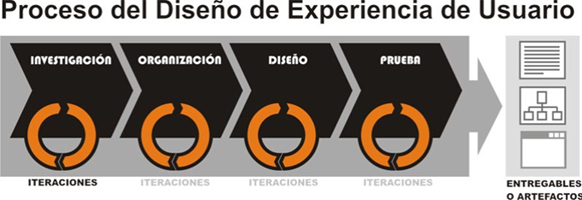
\includegraphics[width=0.5\linewidth]{figuras/proceso_diseno.png}
    \caption{Proceso de Diseño de Experencia de Usuario}
    \label{fig:enter-label}
\end{figure}


\section{Desarrollo Móvil en Android}
\subsection{Razones para elegir Android como plataforma de desarrollo}
Una de las razones principales para elegir Android como plataforma de desarrollo es su alta popularidad Guatemala. Según estudio la mayoría de celulares usados en el país son Samsung y Huawei, los cuales tienen sistema operativo Android \cite{Anonimo2019}.

Según datos recientes, Android domina el tráfico web móvil en el país, con un 82.50\% de participación. Esto significa que la mayoría de los usuarios de dispositivos móviles en Guatemala utilizan este sistema operativo, lo que amplía significativamente el alcance y la accesibilidad del producto desarrollado en esta plataforma \cite{Shum2023}.

\begin{figure} [h]
    \centering
    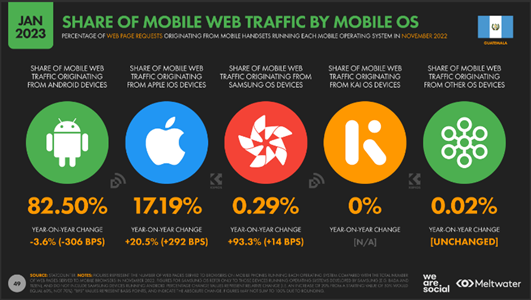
\includegraphics[width=0.5\linewidth]{figuras/mobile_web_traffic.png}
    \caption{Cuota de tráfico web móvil por sistema operativo}
    \label{fig:enter-label}
\end{figure}

Asimismo, Android es conocido por su diversidad en términos de dispositivos, desde teléfonos de alta gama hasta opciones más accesibles. También ofrece un alto nivel de flexibilidad y opciones de personalización, lo que facilita el desarrollo de aplicaciones. Finalmente, el ecosistema de desarrollo de Android está soportado con una vasta cantidad de recursos, herramientas y una comunidad activa de desarrolladores \cite{AnonimoAndroid}.

\subsection{Arquitectura de aplicaciones Android}
La arquitectura de una aplicación Android se basa en el patrón Modelo - Vista - Controlador (MVC). Aunque es muy común utilizar MVVM (Modelo - Vista - \textit{ViewModel}), pues ofrece una separación más clara de la lógica de presentación y facilita el mantenimiento en comparación con MVC \cite{RamosSF}.

\subsubsection{Componentes}
\begin{itemize}
    \item \textbf{Modelo}: Contiene los datos, el estado y la lógica del negocio \cite{Bhadoria2013}.
    \item \textbf{Vista}: Representa la interfaz de usuario. Se comunica con el \textit{ViewModel} a través de mecanismos de enlace de datos (\textit{data binding}), permitiendo una actualización automática de la UI cuando cambian los datos \cite{Bhadoria2013}.
    \item \textbf{\textit{ViewModel}}: Actúa como un intermediario entre el Modelo y la Vista. Expone datos y comandos que la Vista puede consumir y ejecutar, y notifica a la Vista sobre cambios en los datos utilizando observables (como \textit{LiveData}) \cite{Bhadoria2013}.
\end{itemize}

\subsubsection{Flujo de Trabajo}
\begin{itemize}
    \item La Vista se enlaza automáticamente al \textit{ViewModel} para observar los datos \cite{Bhadoria2013}.
    \item El \textit{ViewModel} obtiene los datos del Modelo y prepara la lógica de presentación \cite{Bhadoria2013}.
    \item Cualquier cambio en el Modelo se refleja automáticamente en la Vista a través del \textit{ViewModel} \cite{Bhadoria2013}.
    \item La interacción del usuario en la Vista invoca métodos en el \textit{ViewModel}, que a su vez pueden actualizar el Modelo \cite{Bhadoria2013}.
\end{itemize}

\begin{figure} [H]
    \centering
    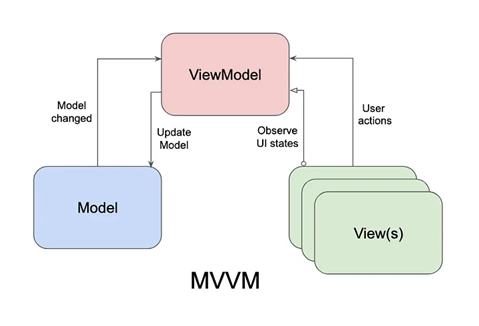
\includegraphics[width=0.5\linewidth]{figuras/mvvm.png}
    \caption{Diagrama de funcionamiento MVVM}
    \label{fig:enter-label}
\end{figure}

\subsection{Buenas prácticas de desarrollo Android}
Al desarrollar aplicaciones para Android, es esencial seguir ciertas buenas prácticas para asegurar la calidad y la eficiencia del producto final \cite{PhillipsStewart2022}:

\subsubsection{Uso de \textit{Layouts} Adecuados}
\begin{itemize}
    \item \textbf{\textit{ConstraintLayout}}: Es eficiente y flexible, permitiendo posicionar elementos de manera relativa a otros elementos \cite{PhillipsStewart2022}.
    \item \textbf{\textit{LinearLayout}}: Organiza los elementos en una sola fila o columna, siendo útil para diseños sencillos y alineaciones básicas \cite{PhillipsStewart2022}.
    \item \textbf{\textit{RelativeLayout}}: Permite posicionar los componentes en relación a otros o a sus propios padres, ofreciendo más flexibilidad pero con un mayor costo de rendimiento comparado con \textit{ConstraintLayout} \cite{PhillipsStewart2022}.
\end{itemize}

\subsubsection{Gestión de Recursos}
\begin{itemize}
    \item Utilizar unidades independientes de densidad (dp) para asegurar que los elementos de la interfaz mantengan su tamaño y proporciones adecuadas en dispositivos con diferentes tamaños de pantalla \cite{PhillipsStewart2022}.
    \item Definir colores, estilos y dimensiones en archivos de recursos para promover la reutilización y mantener la consistencia del diseño \cite{PhillipsStewart2022}.
    \item Utilizar \textit{Gradle} para gestionar dependencias, lo que te permitirá mantener el código actualizado y seguro \cite{PhillipsStewart2022}.
\end{itemize}

\subsubsection{Optimización del Rendimiento}
\begin{itemize}
    \item Minimizar el uso de vistas anidadas para mejorar el rendimiento de la interfaz de usuario \cite{PhillipsStewart2022}.
    \item Evitar operaciones pesadas en el hilo principal \cite{PhillipsStewart2022}.
\end{itemize}

\subsubsection{Seguridad}
\begin{itemize}
    \item Proteger los datos del usuario mediante el uso de almacenamiento cifrado y permisos adecuados \cite{PhillipsStewart2022}.
    \item Validar las entradas del usuario para prevenir ataques de inyección y otras vulnerabilidades de seguridad \cite{PhillipsStewart2022}.
    \item Validar permisos de uso de almacenamiento, cámara, micrófono, etc para respetar las políticas de privacidad de Android \cite{PhillipsStewart2022}.
\end{itemize}

